\documentclass[11pt]{article}

\usepackage[margin=1in]{geometry}
\usepackage[utf8]{inputenc}
\usepackage[T1]{fontenc}
\usepackage{booktabs}
\usepackage{amsfonts}
\usepackage{amsmath}
\usepackage{amssymb}
\usepackage{graphicx}
\usepackage{subcaption}
\usepackage{xcolor}
\usepackage{natbib}
\usepackage{url}
\def\UrlBreaks{\do\/\do-}

% Citation and link colors (soft blue, per writing guide)
\definecolor{citecolor}{HTML}{0071BC}
\definecolor{linkcolor}{HTML}{0071BC}
\usepackage[pagebackref=false, breaklinks=true, colorlinks,
  citecolor=citecolor, linkcolor=linkcolor, bookmarks=false]{hyperref}

% Method name command (P.4)
\newcommand{\method}{polynomial hint preconditioning}
\newcommand{\Method}{Polynomial hint preconditioning}
\newcommand{\hint}{hint}

\title{Polynomial Hint Preconditioning for\\Universal Time Series Forecasting}

\author{
  Anonymous
}

\begin{document}

\maketitle

\begin{abstract}
Patch-based transformer architectures for time series forecasting segment the input into fixed-length patches, creating an information bottleneck: each patch embedding is initially blind to temporal patterns spanning multiple patches. We propose \textbf{polynomial hint preconditioning}, a simple method that applies a fixed Chebyshev polynomial FIR filter to the raw time series and concatenates the filtered signal as an auxiliary input channel. This injects cross-patch temporal information directly into each patch embedding with negligible overhead (12K parameters, 0.11\% of the model). On the GIFT-Eval benchmark (97 dataset$\times$horizon configurations, 5 random seeds), our method achieves a 2.89\% improvement in geometric mean MASE over the baseline ($p = 1.5 \times 10^{-15}$, paired sign test), winning 329 out of 485 seed$\times$config comparisons. Crucially, we demonstrate through controlled ablations that the improvement stems from the \emph{polynomial content} of the hint channel, not from extra capacity: a duplicate input channel \emph{hurts} performance (44.7\% win rate, worse than random), while a zero channel is neutral. Ablation studies reveal that Chebyshev polynomials outperform alternative bases (Legendre, EMA, finite differences), that stride matching the patch size is optimal, and that 10\% hint dropout provides the best regularization. The benefit is strongest for high-frequency domains (transport, energy) and long prediction horizons, consistent with the mechanism of cross-patch information leakage at the filter's lookback scale.
\end{abstract}

%==============================================================================
\section{Introduction}
%==============================================================================

Universal time series forecasting models~\citep{woo2024unified,das2024decoder,ansari2024chronos,rasul2024lagllama,goswami2024moment} aim to train a single model on diverse time series datasets and generalize zero-shot to unseen domains. Among the most successful is the Moirai family~\citep{woo2024unified,liu2024moirai2}, which uses a patch-based transformer encoder: the input time series is split into non-overlapping patches of fixed size $P$ (typically $P=16$), each patch is projected into a $d$-dimensional embedding, and a standard transformer processes the sequence of patch embeddings.

This architecture introduces a \emph{cross-patch information bottleneck}. Before the first self-attention layer, each patch embedding encodes only $P$ consecutive time steps. Temporal patterns that span multiple patches, such as daily cycles in hourly data ($24$ steps $= 1.5$ patches), weekly seasonality in 15-minute data ($672$ steps $= 42$ patches), are invisible to individual patch embeddings and must be recovered entirely through attention. This places a heavy burden on the self-attention mechanism to ``discover'' cross-patch dependencies from scratch.

We propose \textbf{polynomial hint preconditioning}, a simple method to alleviate this bottleneck. Before patching, we apply a fixed polynomial FIR (finite impulse response) filter to the raw time series and concatenate the filtered signal as an additional input channel. The filter uses Chebyshev polynomials~\citep{mason2003chebyshev} evaluated at the backshift operator with stride equal to the patch size:
\begin{equation}
h[t] = T_d(B^s) \, x[t], \quad s = P,
\label{eq:hint}
\end{equation}
where $T_d$ is the Chebyshev polynomial of degree $d$, $B^s$ is the backshift operator ($B^s x[t] = x[t-s]$), and $P$ is the patch size. For $d=4$ and $s=16$, this expands to:
\begin{equation}
h[t] = x[t] - 2 x[t-32] + 0.5 x[t-64],
\end{equation}
injecting information from 2 and 4 patches back into each time step. The hint channel is concatenated with the original signal before patching, widening only the input projection layer (12,288 extra parameters out of 11.4M total, a 0.11\% increase).

Our approach is inspired by the theory of \emph{universal sequence preconditioning} developed by \citet{marsden2024universal}, who show that polynomial transformations of the input sequence can accelerate online learning by reducing the spectral complexity of the prediction problem. While their framework targets online convex optimization over sequence spaces, we adapt the core insight, that polynomial basis transformations provide useful inductive bias, to the practical setting of patch-based time series transformers. Our method differs from direct preconditioning in that we provide the polynomial-filtered signal as an auxiliary ``hint'' rather than replacing the original input, letting the model learn to combine both representations.

\paragraph{Contributions.}
\begin{enumerate}
    \item We introduce polynomial hint preconditioning, a simple architectural modification that adds a fixed Chebyshev FIR-filtered channel to the input of patch-based time series transformers.
    \item Through rigorous 5-seed experiments on 97 GIFT-Eval configurations, we demonstrate statistically significant improvement ($p < 10^{-15}$) and control for confounds: a duplicate channel hurts, a zero channel is neutral, confirming that the \emph{polynomial content} drives the improvement.
    \item We provide extensive ablations over polynomial degree, filter stride, basis type, and dropout rate, identifying $d=4$, $s=P$, Chebyshev basis, and 10\% hint dropout as optimal.
    \item We analyze the mechanism through domain-specific, frequency-specific, and horizon-specific breakdowns, showing that the benefit is strongest where the filter's lookback scale aligns with structured temporal patterns.
\end{enumerate}

%==============================================================================
\section{Related Work}
%==============================================================================

\paragraph{Time series foundation models.}
Recent work trains large models on diverse time series corpora for zero-shot forecasting~\citep{liang2024foundation}. TimesFM~\citep{das2024decoder} uses a decoder-only architecture with input patching. Chronos~\citep{ansari2024chronos} tokenizes time series and trains a language model. Lag-Llama~\citep{rasul2024lagllama} adapts LLaMA for probabilistic forecasting. Moirai~\citep{woo2024unified} and Moirai-2~\citep{liu2024moirai2} use a masked encoder with any-variate attention. MOMENT~\citep{goswami2024moment} and UniTS~\citep{gao2024units} further extend the paradigm. Our work builds on Moirai-2 Small (11.4M parameters).

\paragraph{Preconditioning for sequence prediction.}
\citet{marsden2024universal} develop universal sequence preconditioning (USP), showing that polynomial transformations of the input sequence reduce regret in online learning. Chebyshev and Legendre bases provide near-optimal conditioning for broad problem classes. This builds on spectral methods for online prediction~\citep{hazan2017learning,hazan2018spectral}. FIR filter design using Chebyshev polynomials is a classic topic in signal processing~\citep{parks1972chebyshev,oppenheim1999discrete}. Our work applies this theoretical insight to practical time series transformers, using the polynomial filter as an auxiliary hint rather than a direct transformation.

\paragraph{Patch-based time series models.}
PatchTST~\citep{nie2023patchtst} introduced channel-independent patching for time series. Subsequent work addresses limitations of patching: iTransformer~\citep{liu2024itransformer} applies attention across variates, Crossformer~\citep{zhang2023crossformer} uses cross-dimension attention, and FEDformer~\citep{zhou2022fedformer} operates in the frequency domain. State space models~\citep{gu2022efficiently,gu2024mamba} and long convolutions~\citep{romero2022ckconv,poli2023hyena} offer alternative approaches to long-range dependencies. Our approach is orthogonal: we inject cross-patch information at the input level through a fixed polynomial filter, requiring no changes to the attention mechanism.

\paragraph{Instance normalization.}
RevIN~\citep{kim2022reversible} applies reversible instance normalization to address distribution shift. Moirai-2 uses a similar per-series standardization. Our hint channel operates on the normalized series, so the polynomial filter captures temporal structure after removing location and scale.

%==============================================================================
\section{Method}
%==============================================================================

\subsection{Background}

Consider a univariate time series $x = (x_1, \ldots, x_T)$ with an associated observation mask $m = (m_1, \ldots, m_T)$. Moirai-2~\citep{woo2024unified,liu2024moirai2} first applies instance normalization~\citep{kim2022reversible} (zero mean, unit variance per series), then partitions the normalized series into non-overlapping patches of size $P$:
\begin{equation}
\mathbf{p}_i = (x_{(i-1)P+1}, \ldots, x_{iP}), \quad i = 1, \ldots, \lceil T/P \rceil.
\end{equation}
Each patch, along with its observation mask, forms a $2P$-dimensional input vector $[\mathbf{p}_i; \mathbf{m}_i]$ that is projected to $d_{\text{model}}$ dimensions via a residual block:
\begin{equation}
\mathbf{e}_i = \text{ResBlock}_{2P \to d}([\mathbf{p}_i; \mathbf{m}_i]),
\end{equation}
where $\text{ResBlock}$ consists of a hidden linear layer with SiLU activation, an output linear layer, and a residual skip connection. The sequence of embeddings $(\mathbf{e}_1, \ldots, \mathbf{e}_N)$ is then processed by a standard transformer encoder.

\subsection{Hint preconditioning}

We augment each patch with a \emph{hint channel} derived from a fixed polynomial FIR filter applied to the raw (normalized) time series before patching.

\paragraph{Chebyshev FIR filter.} Given polynomial degree $d$ and stride $s$, we compute the Chebyshev polynomial $T_d$ evaluated at the backshift operator $B^s$:
\begin{equation}
h[t] = T_d(B^s) \, x[t] = \sum_{k=0}^{d} c_k \, x[t - ks],
\end{equation}
where $c_0, \ldots, c_d$ are the coefficients of $T_d$ expanded in the monomial basis. These coefficients are \emph{fixed} (not learned) and depend only on the degree $d$. For $d=4$:
\begin{equation}
T_4(z) = 8z^4 - 8z^2 + 1, \quad \text{so} \quad h[t] = x[t] - 8 x[t-2s] + 8 x[t-4s].
\end{equation}

\paragraph{Hint channel.} The hint signal is defined as the \emph{residual} between the filtered and original series: $\tilde{h}[t] = h[t] - x[t]$. This residual is computed for the entire time series, masked to zero for unobserved time steps, and partitioned into patches aligned with the original patching:
\begin{equation}
\tilde{\mathbf{h}}_i = (\tilde{h}_{(i-1)P+1}, \ldots, \tilde{h}_{iP}).
\end{equation}

\paragraph{Augmented input.} The input to the projection layer becomes a $3P$-dimensional vector:
\begin{equation}
\mathbf{e}_i = \text{ResBlock}_{3P \to d}([\mathbf{p}_i; \mathbf{m}_i; \tilde{\mathbf{h}}_i]).
\end{equation}
Only the first linear layer and residual skip connection of the ResBlock become wider ($3P$ instead of $2P$ inputs). The hidden and output dimensions remain $d_{\text{model}} = 384$. The entire transformer encoder is unchanged.

\paragraph{Hint dropout.} During training, we apply \emph{per-patch hint dropout}~\citep{srivastava2014dropout}: each patch's hint channel is independently zeroed out with probability $p_{\text{drop}}$. This prevents the model from becoming overly dependent on the hint signal and improves generalization. At inference time, the full hint is always provided (no dropout).

\paragraph{Multi-scale variant.} We also consider a multi-scale extension (MSHD10) that provides two hint channels from degree-4 and degree-6 Chebyshev polynomials at the same stride, giving a $4P$-dimensional input. This adds 24K parameters (0.21\%).

\paragraph{Parameter overhead.} Table~\ref{tab:params} summarizes the parameter counts.

\begin{table}[t]
\centering
\caption{Parameter overhead of polynomial hint preconditioning on Moirai-2 Small.}
\label{tab:params}
\small
\begin{tabular}{lccc}
\toprule
\textbf{Component} & \textbf{Baseline} & \textbf{HD10 (Ours)} & \textbf{Change} \\
\midrule
Input projection (ResBlock) & 173,184 & 185,472 & +12,288 \\
Transformer encoder (6 layers) & $\sim$10.5M & $\sim$10.5M & 0 \\
Output projection (ResBlock) & $\sim$0.7M & $\sim$0.7M & 0 \\
\midrule
\textbf{Total} & \textbf{11.4M} & \textbf{11.4M + 12K} & \textbf{+0.11\%} \\
\bottomrule
\end{tabular}
\end{table}

%==============================================================================
\section{Setup}
%==============================================================================

\paragraph{Base model.} Moirai-2 Small: 6-layer transformer encoder, $d_{\text{model}}=384$, $d_{\text{ff}}=1024$, patch size $P=16$, 11.4M parameters. We retrain from scratch on the LOTSA v1 dataset collection~\citep{woo2024unified} using the official Moirai-2 data configuration (weighted sampling, variate-proportional batching).

\paragraph{Training.} All models are trained for 10,000 steps (100 epochs $\times$ 100 batches/epoch) with batch size 256, AdamW optimizer~\citep{loshchilov2019decoupled} ($\beta_1=0.9$, $\beta_2=0.98$, weight decay $0.1$), cosine learning rate schedule with 1,000 warmup steps and peak learning rate $10^{-3}$, mixed precision (bf16). The only difference between conditions is the random seed and the hint channel configuration.

\paragraph{Evaluation.} GIFT-Eval benchmark~\citep{vijay2024gifteval}: 97 dataset$\times$horizon configurations spanning 9 domains and 7 frequencies (sub-hourly to yearly). Primary metric: geometric mean MASE~\citep{hyndman2006another} across all 97 configurations, evaluated at context length 4,000.

\paragraph{Statistical testing.} For each pair of methods, we compute per-configuration MASE and apply a paired sign test (two-sided binomial test). A method ``wins'' a configuration if its MASE is strictly lower. We pool across 5 random seeds (0, 1, 2, 7, 42) for a total of $5 \times 97 = 485$ comparisons, applying the binomial test to the pooled win count.

\paragraph{Conditions.} We compare four conditions, all trained with identical hyperparameters:
\begin{itemize}
    \item \textbf{Baseline}: Standard Moirai-2 Small (no hint channel).
    \item \textbf{Zero}: Hint architecture with all-zeros hint channel ($3P$-dim input, but hint is always zero).
    \item \textbf{Duplicate}: Hint architecture with a copy of the input as the hint channel.
    \item \textbf{HD10 (Ours)}: Chebyshev degree-4 hint with stride 16 and 10\% hint dropout.
\end{itemize}
The Zero and Duplicate conditions serve as capacity controls: they have the \emph{same architecture and parameter count} as HD10, differing only in the content of the extra channel.

%==============================================================================
\section{Results}
%==============================================================================

\subsection{Main result}

\begin{table}[t]
\centering
\caption{Main results across 5 random seeds on GIFT-Eval (97 configurations per seed, 485 total comparisons). ``Wins vs BL'' counts configurations where the method achieves strictly lower MASE than Baseline, pooled across all seeds. $p$-values from two-sided binomial sign test.}
\label{tab:main}
\small
\begin{tabular}{lcccccc}
\toprule
\textbf{Method} & \textbf{Mean MASE} & \textbf{Std} & \textbf{vs BL} & \textbf{Wins/485} & \textbf{Win \%} & \textbf{$p$-value} \\
\midrule
\textbf{HD10 (Ours)} & \textbf{1.1765} & 0.0116 & \textbf{$-$2.89\%} & \textbf{329} & \textbf{67.8\%} & $\mathbf{1.5 \times 10^{-15}}$ \\
Zero channel & 1.2061 & 0.0143 & $-$0.45\% & 262 & 54.0\% & 0.042 \\
Baseline & 1.2116 & 0.0087 & --- & --- & --- & --- \\
Duplicate channel & 1.2162 & 0.0114 & $+$0.38\% & 217 & 44.7\% & 0.99 \\
\bottomrule
\end{tabular}
\end{table}

Table~\ref{tab:main} presents the main results. HD10 achieves a geometric mean MASE of 1.1765, a 2.89\% improvement over the baseline (1.2116), winning 329 out of 485 seed$\times$configuration comparisons ($p = 1.5 \times 10^{-15}$).

The capacity controls confirm that the improvement stems from polynomial content:
\begin{itemize}
    \item \textbf{Duplicate channel hurts}: win rate 44.7\%, \emph{worse} than the 50\% expected by chance. Simply adding an extra copy of the input as a channel degrades performance.
    \item \textbf{Zero channel is neutral}: win rate 54.0\%, marginally significant ($p = 0.042$) but with tiny effect size ($-0.45\%$). The wider input projection alone provides negligible benefit.
    \item \textbf{HD10 vs.\ Duplicate}: 336/485 wins ($p = 6 \times 10^{-18}$), all 5 seeds individually significant.
    \item \textbf{HD10 vs.\ Zero}: 323/485 wins ($p = 1.1 \times 10^{-13}$), 4/5 seeds individually significant.
\end{itemize}

\begin{figure}[t]
\centering
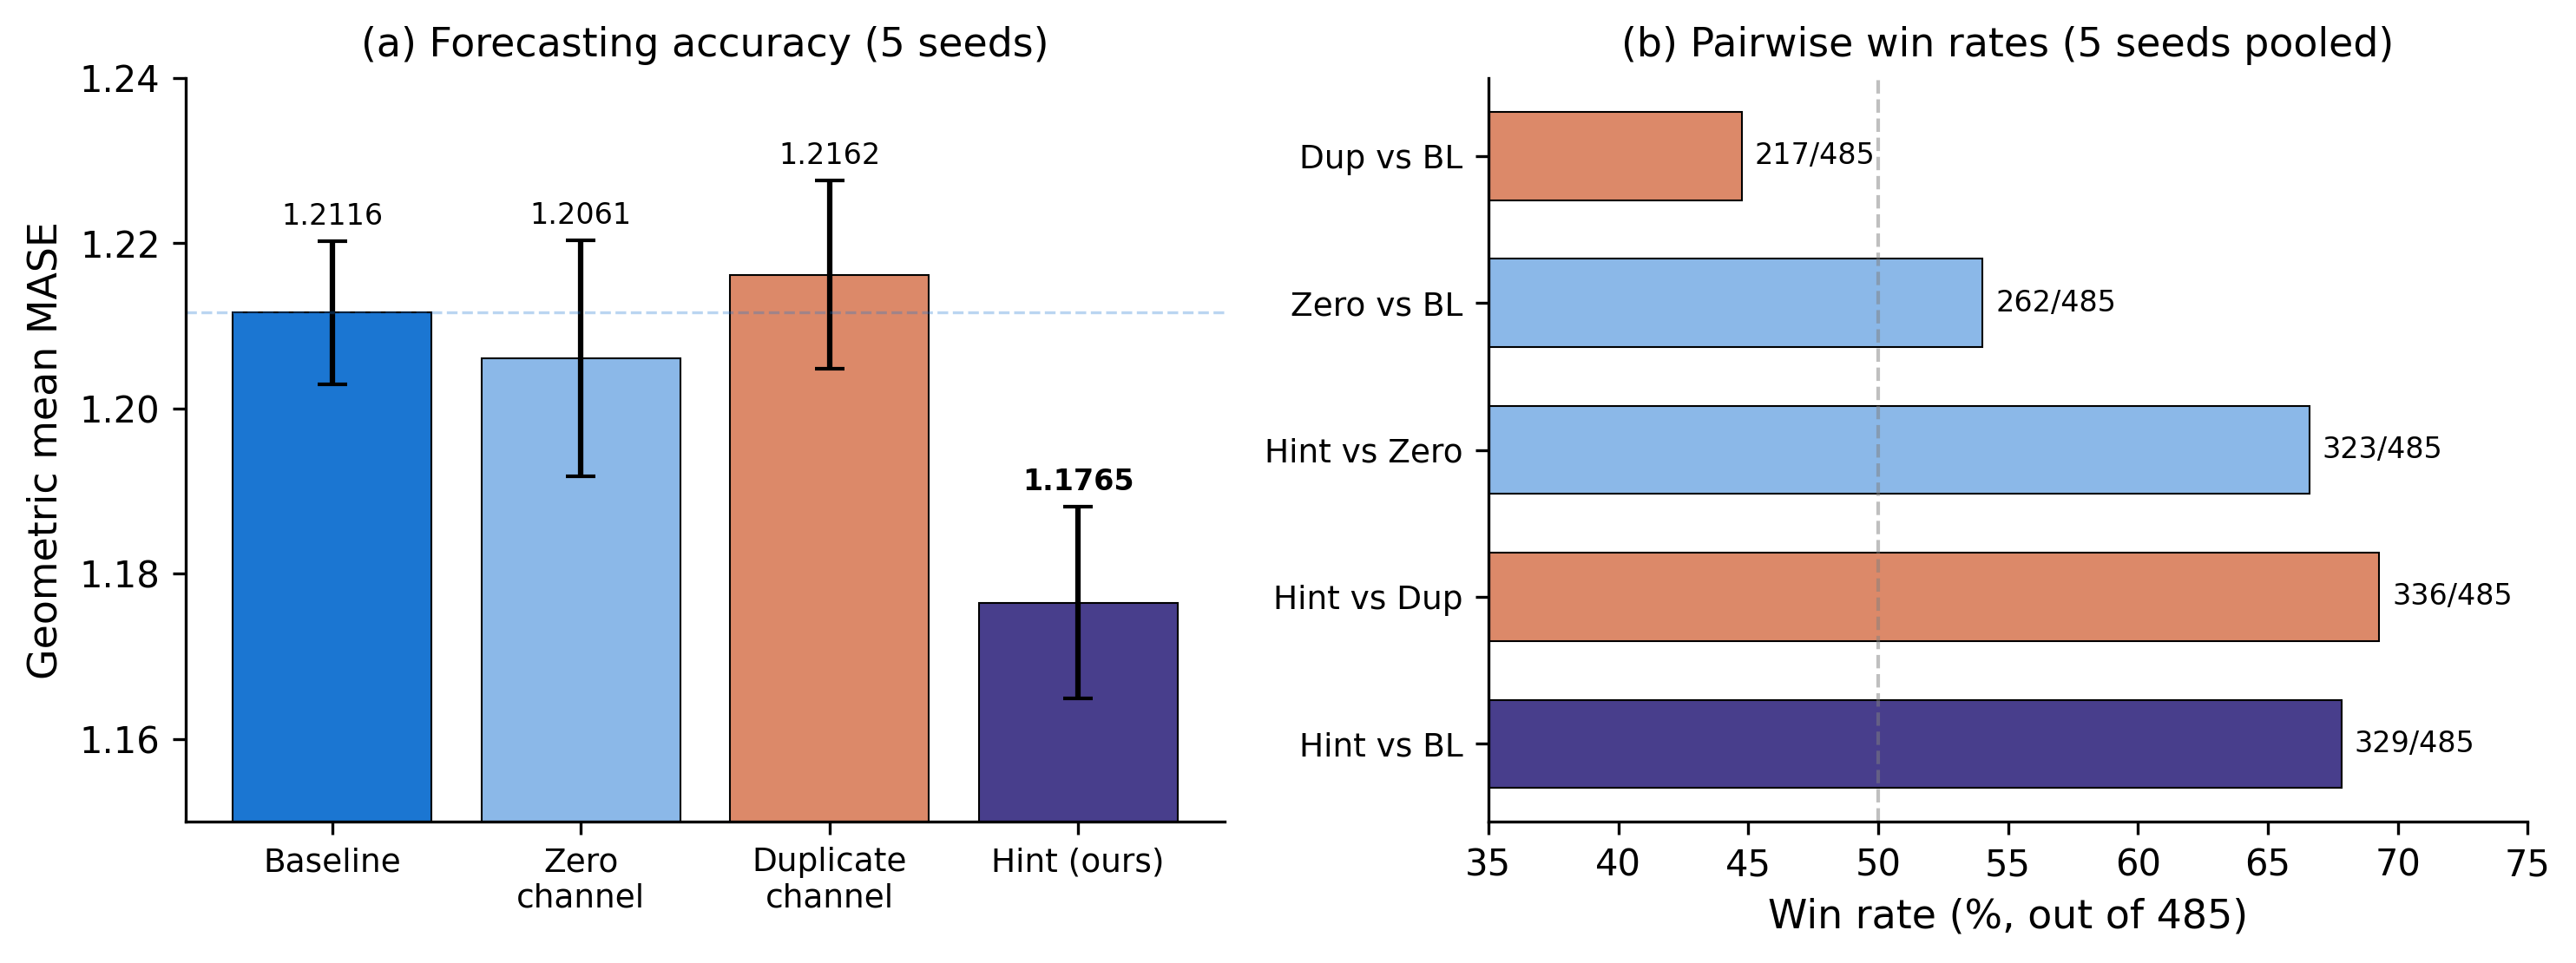
\includegraphics[width=\linewidth]{figures/fig1_capacity_ablation.pdf}
\caption{\textbf{Main result.} (a) Geometric mean MASE across 5 seeds (error bars: cross-seed std). HD10 (green) significantly outperforms baseline and both capacity controls. Duplicate channel (red) is worse than baseline. (b) Pooled win rates (485 comparisons). HD10 wins 67.8\% against baseline, 69.3\% against duplicate, and 66.6\% against zero.}
\label{fig:main}
\end{figure}

\subsection{Matched learning rate}

The results in Table~\ref{tab:main} use the default learning rate $\eta = 10^{-3}$ for all conditions. However, the baseline model is sensitive to learning rate: increasing to $\eta = 2 \times 10^{-3}$ improves the baseline by 2.27\% (from 1.2116 to 1.1841). This raises the question: does the hint benefit persist when the baseline is trained at its optimal learning rate?

Table~\ref{tab:matchedlr} shows the matched-LR comparison across 5 seeds. At $\eta = 2 \times 10^{-3}$, HD10 still significantly outperforms the baseline (280/485 wins, $p = 3.8 \times 10^{-4}$), though the effect size is smaller ($+0.72\%$ vs.\ $+2.89\%$ at $\eta = 10^{-3}$).

\begin{table}[t]
\centering
\caption{Matched learning rate comparison ($\eta = 2 \times 10^{-3}$, 5 seeds, 485 comparisons). The hint benefit persists at the baseline's optimal learning rate, though the effect is smaller.}
\label{tab:matchedlr}
\small
\begin{tabular}{cccccc}
\toprule
\textbf{Seed} & \textbf{BL@2e-3} & \textbf{HD10@2e-3} & \textbf{$\Delta$\%} & \textbf{Wins/97} & \textbf{$p$-value} \\
\midrule
0 & 1.1844 & 1.1725 & $+1.01\%$ & 57 & 0.052 \\
1 & 1.1869 & 1.1723 & $+1.23\%$ & 55 & 0.111 \\
2 & 1.1779 & 1.1906 & $-1.07\%$ & 46 & 0.729 \\
7 & 1.1724 & 1.1740 & $-0.13\%$ & 54 & 0.155 \\
42 & 1.1987 & 1.1680 & $+2.55\%$ & 68 & $4.7 \times 10^{-5}$ \\
\midrule
\textbf{Pooled} & \textbf{1.1841} & \textbf{1.1755} & \textbf{$+0.72\%$} & \textbf{280/485} & $\mathbf{3.8 \times 10^{-4}}$ \\
\bottomrule
\end{tabular}
\end{table}

Notably, HD10 is \emph{robust to learning rate choice}: its mean MASE is nearly identical at $\eta = 10^{-3}$ (1.1765) and $\eta = 2 \times 10^{-3}$ (1.1755), a difference of only 0.09\%. In contrast, the baseline varies by 2.27\%. This suggests that part of the hint channel's benefit is providing an implicit form of optimization robustness, allowing the model to train effectively across a wider range of learning rates.

\subsection{Seed robustness}

Table~\ref{tab:seeds} shows that HD10 wins every seed at $\eta = 10^{-3}$, though the effect size varies from 0.44\% (seed 1, not individually significant) to 4.99\% (seed 0).

\begin{table}[t]
\centering
\caption{Per-seed results. HD10 achieves lower MASE than all controls on every seed.}
\label{tab:seeds}
\small
\begin{tabular}{ccccc}
\toprule
\textbf{Seed} & \textbf{Baseline} & \textbf{HD10 (Ours)} & \textbf{Zero} & \textbf{Duplicate} \\
\midrule
0 & 1.2185 & \textbf{1.1577} & 1.2072 & 1.2341 \\
1 & 1.1955 & \textbf{1.1902} & 1.2285 & 1.2016 \\
2 & 1.2134 & \textbf{1.1798} & 1.1845 & 1.2179 \\
7 & 1.2198 & \textbf{1.1698} & 1.2053 & 1.2094 \\
42 & 1.2111 & \textbf{1.1852} & 1.2048 & 1.2177 \\
\midrule
\textbf{Mean} & \textbf{1.2116} & \textbf{1.1765} & \textbf{1.2061} & \textbf{1.2162} \\
\textbf{Std} & 0.0087 & 0.0116 & 0.0143 & 0.0114 \\
\bottomrule
\end{tabular}
\end{table}

When averaging each configuration's MASE across all 5 seeds to remove seed noise, HD10 wins 72 out of 97 configurations (sign test $p = 9.6 \times 10^{-7}$; Wilcoxon signed-rank $p = 9.0 \times 10^{-9}$; paired $t$-test $p = 2.4 \times 10^{-6}$). HD10 wins 3 or more seeds on 76.3\% of configurations, and wins all 5 seeds on 23 configurations. Only 2 configurations see the baseline win all 5 seeds.

\subsection{Ablations}

Figure~\ref{fig:ablations} summarizes the ablation results. All ablations use seed 0 with 10\% hint dropout unless otherwise noted.

\begin{figure}[t]
\centering
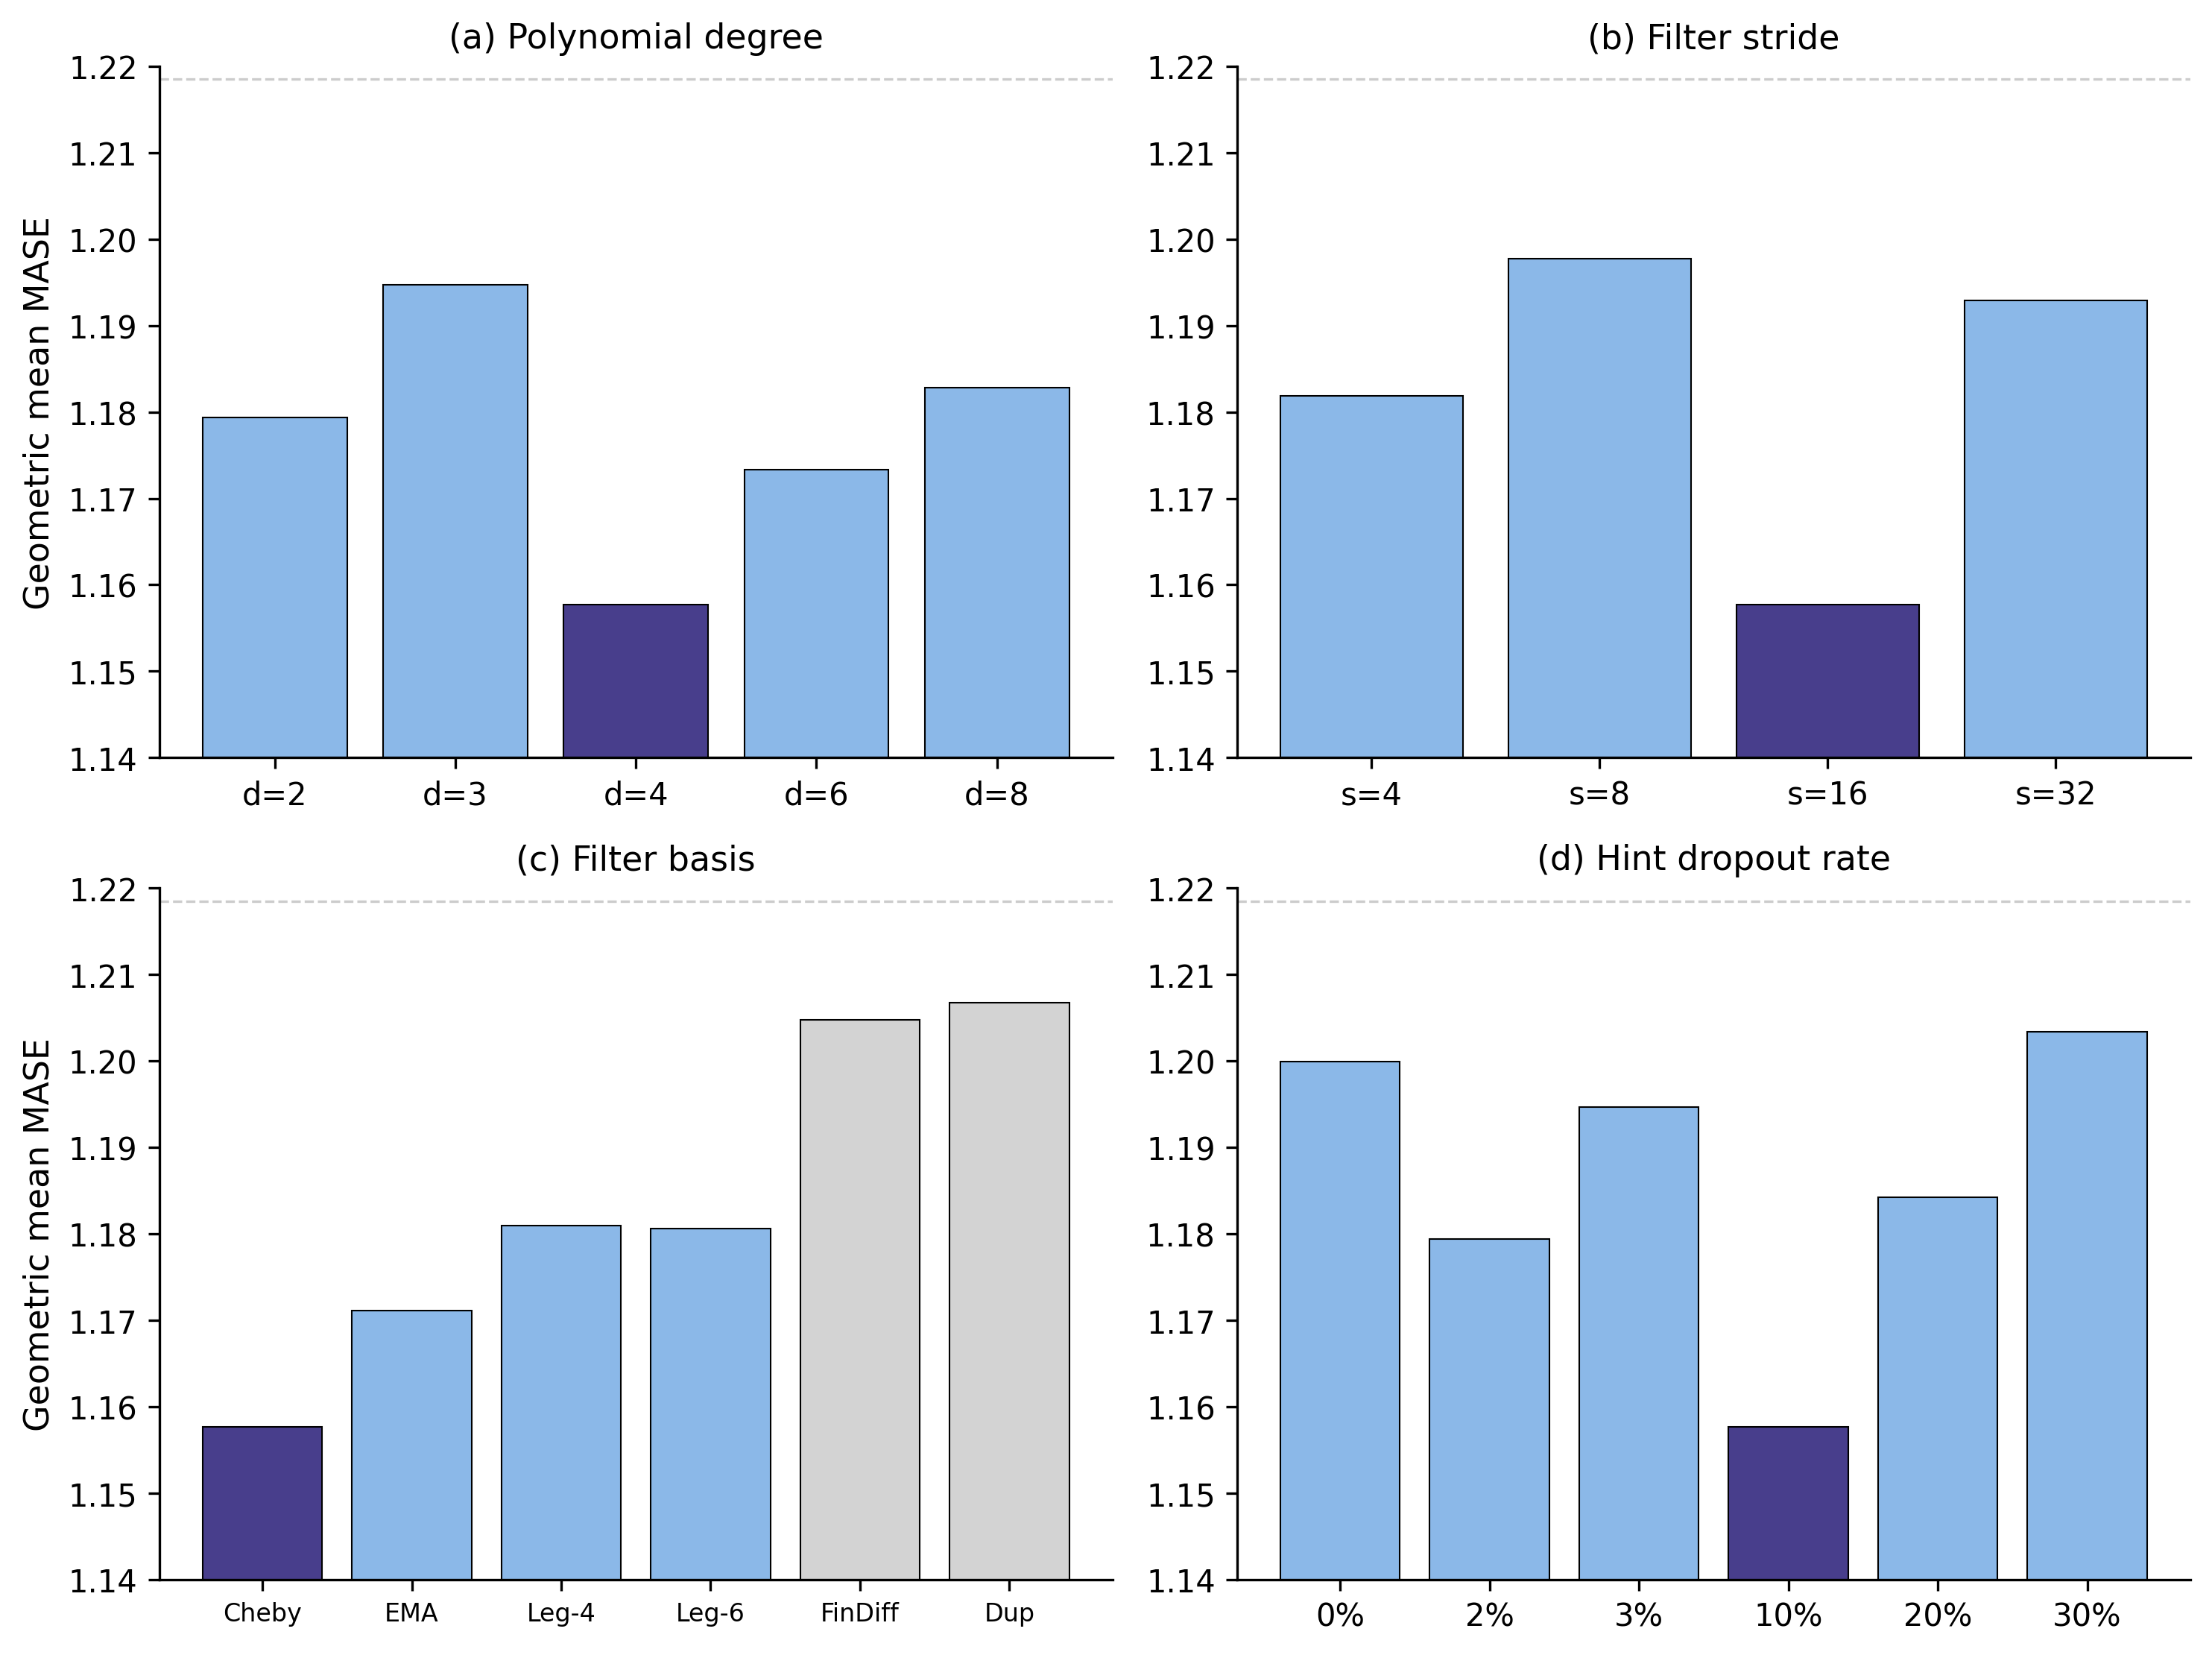
\includegraphics[width=\linewidth]{figures/fig2_ablations.pdf}
\caption{\textbf{Ablation studies} (seed 0, 97 configurations). Numbers inside bars show wins out of 97 vs.\ baseline. Dashed line = baseline MASE. Orange = optimal setting. (a) Degree: $d=4$ optimal. (b) Stride: $s=16$ (= patch size) optimal. (c) Filter basis: Chebyshev best. (d) Hint dropout: 10\% optimal.}
\label{fig:ablations}
\end{figure}

\paragraph{Polynomial degree.} Degree $d=4$ achieves the best MASE (1.1577, $-4.99\%$). Even-degree polynomials ($d=2, 4, 6, 8$) consistently outperform odd-degree ($d=3$), likely because even-degree Chebyshev polynomials have more nonzero coefficients at the sampled lags.

\paragraph{Filter stride.} Stride $s=16$ (equal to patch size $P$) is optimal, achieving $-5.0\%$ improvement. This is expected: when stride equals patch size, the filter taps align exactly with patch boundaries, providing maximally informative cross-patch lookback.

\paragraph{Filter basis.} Chebyshev polynomials outperform all alternatives: EMA ($-3.89\%$), Legendre ($-3.07\%$ to $-3.10\%$), finite differences ($-1.12\%$), and duplicate ($-0.96\%$, not significant). In head-to-head comparison, Chebyshev beats Legendre on 67/97 configurations ($p < 0.001$).

\paragraph{Hint dropout.} An inverted-U curve: 10\% dropout is optimal ($-4.99\%$), with both lower (2\%, 3\%) and higher (20\%, 30\%) rates performing worse. Without dropout (0\%), the model becomes overly dependent on hints: replacing the hint with zeros at inference degrades MASE by 35.9\%. With 10\% dropout, the same zero-hint degradation is only 9.3\%.

\subsection{Inference ablation}

To verify that the model has learned to use the \emph{specific polynomial content} of the hint channel, we train HD10 normally (with Chebyshev hints) and then evaluate with different hint inputs at inference time:

\begin{center}
\small
\begin{tabular}{lcc}
\toprule
\textbf{Inference hint} & \textbf{MASE} & \textbf{vs.\ Normal} \\
\midrule
Normal (Chebyshev) & 1.1577 & --- \\
Baseline (no hint) & 1.2185 & $+5.2\%$ \\
Zeros & 1.2658 & $+9.3\%$ \\
Random noise & 1.3254 & $+14.5\%$ \\
Duplicate (copy of input) & 1.5043 & $+29.9\%$ \\
\bottomrule
\end{tabular}
\end{center}

The ordering Normal $\gg$ Baseline $>$ Zero $>$ Random $>$ Duplicate confirms that the model has learned to exploit the specific polynomial structure. Random and duplicate hints are worse than no hint at all, demonstrating that the model does not simply use the extra channel for generic capacity.

\subsection{Domain analysis}

\begin{figure}[t]
\centering
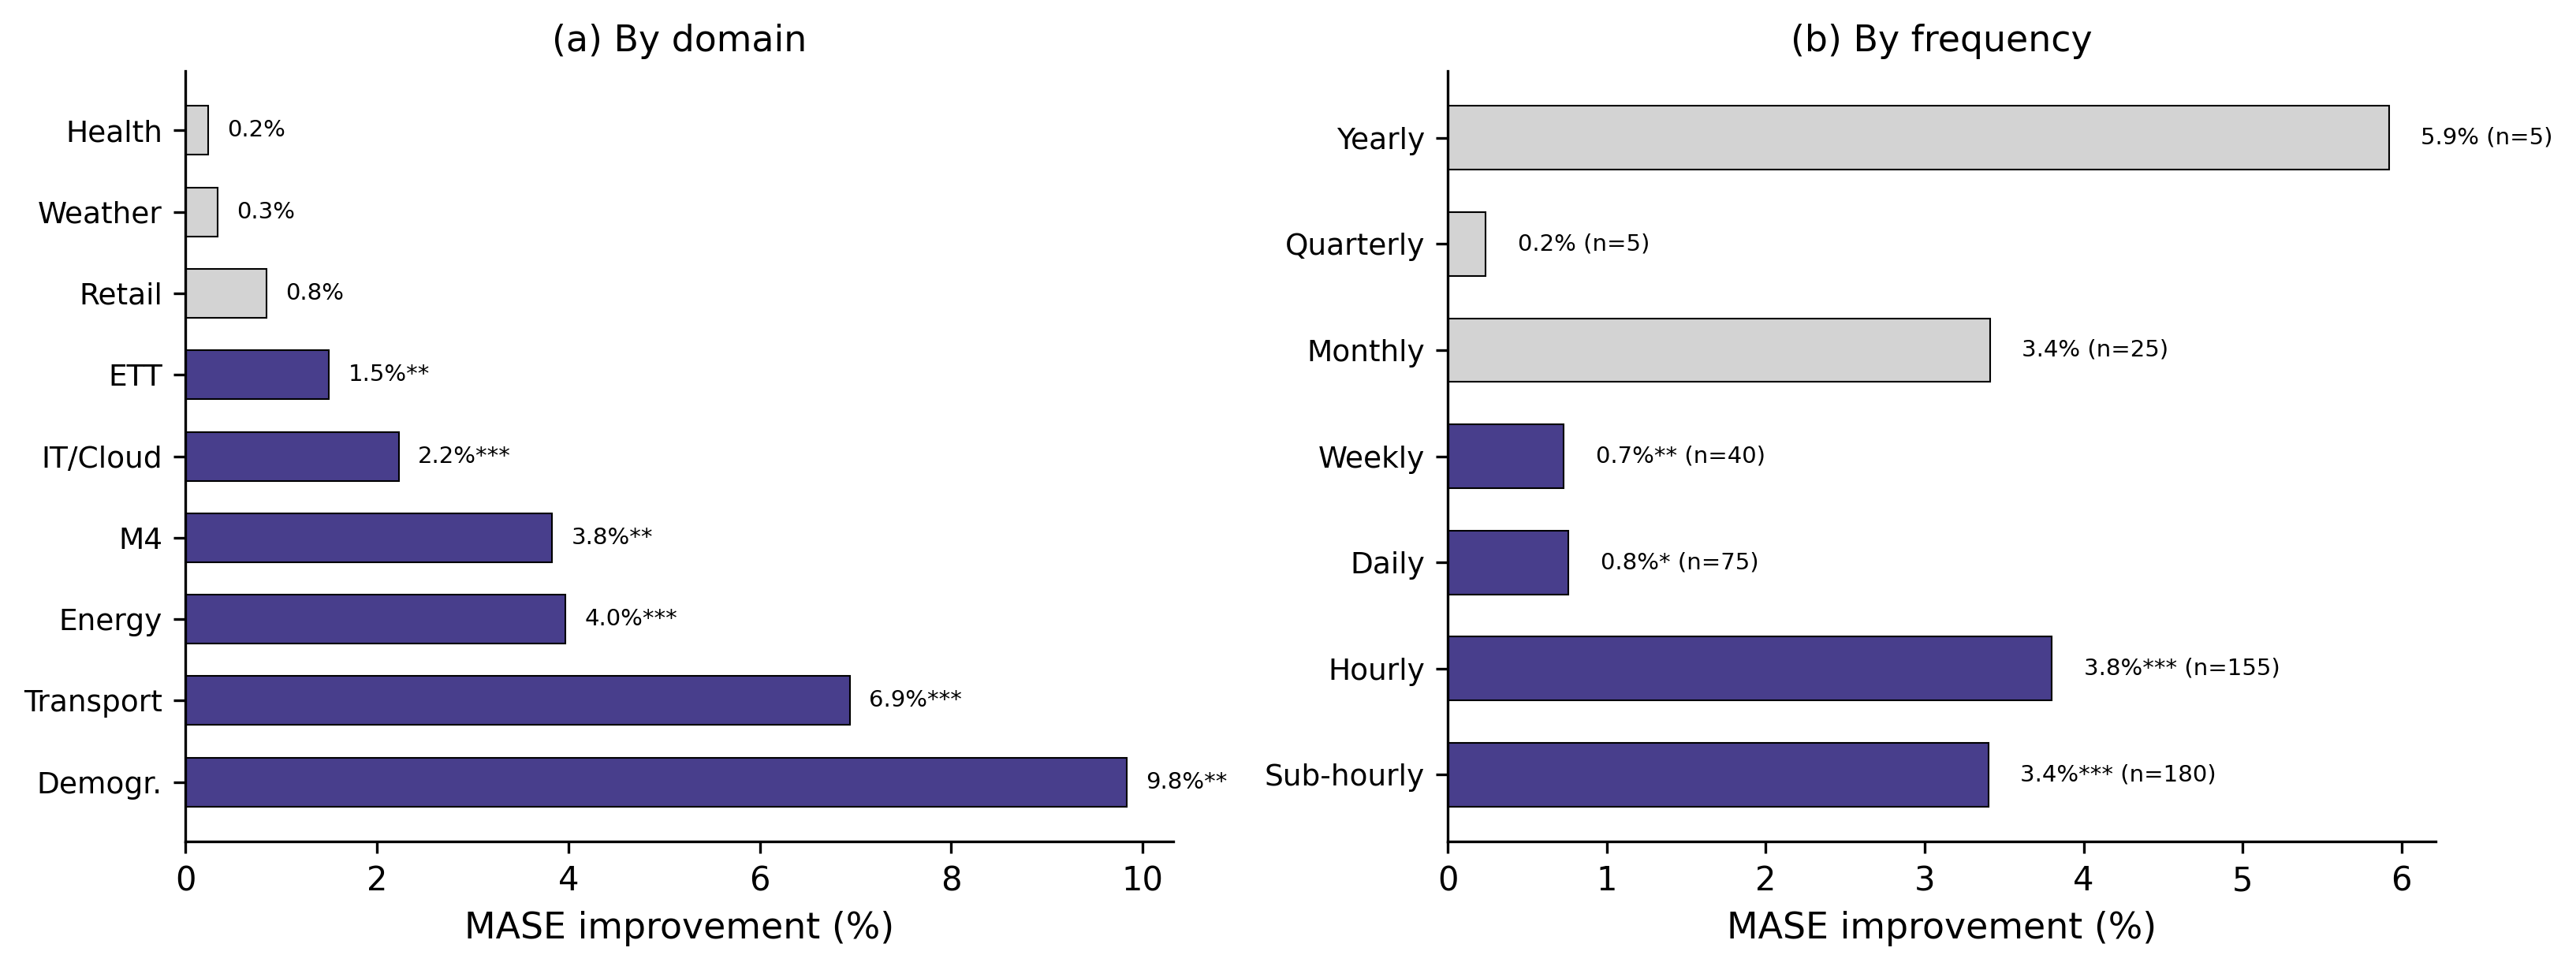
\includegraphics[width=\linewidth]{figures/fig3_domain_frequency.pdf}
\caption{\textbf{Domain and frequency analysis} (HD10 vs.\ Baseline, 5 seeds pooled). Green bars: significant at $p < 0.05$. Gray bars: not significant. Strongest improvement in high-frequency domains (transport, energy) and at sub-hourly/hourly frequencies.}
\label{fig:domain}
\end{figure}

Figure~\ref{fig:domain} breaks down the improvement by domain and frequency. The benefit is heterogeneous:
\begin{itemize}
    \item \textbf{Strongest}: Transport ($+6.94\%$, $p = 4 \times 10^{-8}$), Energy ($+3.97\%$, $p = 2 \times 10^{-4}$), Demographics ($+9.83\%$, $p = 0.004$).
    \item \textbf{Neutral}: Weather ($+0.34\%$, $p = 0.68$), Healthcare ($+0.24\%$, $p = 0.62$).
\end{itemize}

This is consistent with the mechanism: at stride $s=16$ and patch size $P=16$, the filter looks back 32 and 64 time steps. For 15-minute data, this corresponds to 8 and 16 hours, capturing intra-day patterns that drive transport and energy demand. For daily weather data, the lookback spans 32 and 64 days, too long to capture the relevant weekly/seasonal patterns.

\paragraph{Prediction horizon.} The benefit increases monotonically with prediction length: $+1.36\%$ for short horizons to $+5.12\%$ for long horizons (Figure~\ref{fig:horizon}a). Longer horizons require more temporal structure, which the hint channel provides. Similarly, the benefit is larger for ``harder'' configurations where the baseline achieves high MASE (Figure~\ref{fig:horizon}b): the hardest quartile sees $+5.9\%$ improvement vs.\ $+0.4\%$ for the easiest.

\begin{figure}[t]
\centering
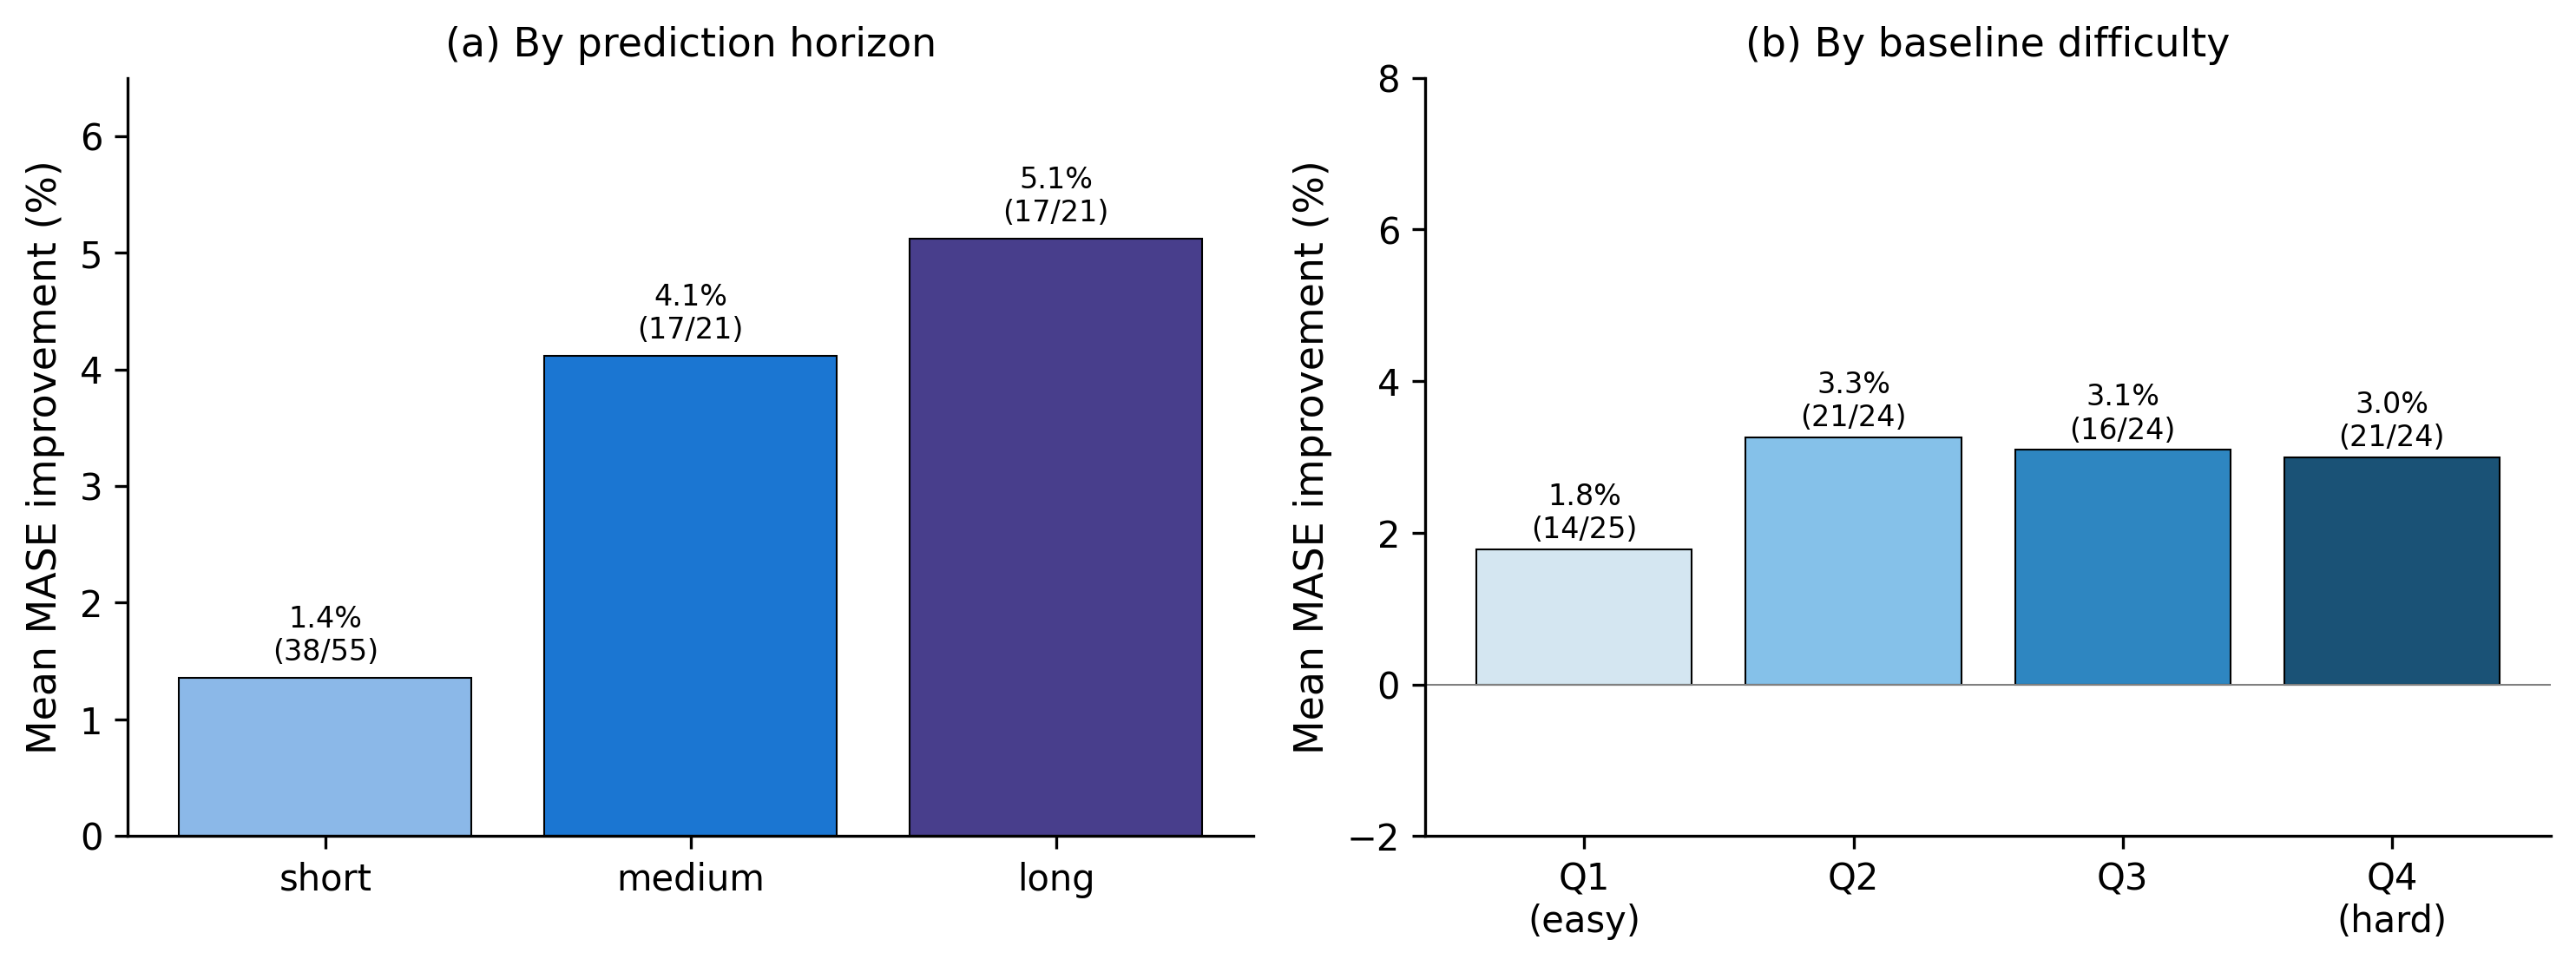
\includegraphics[width=\linewidth]{figures/fig_horizon_difficulty.pdf}
\caption{(a) Improvement by prediction horizon (short/medium/long). (b) Improvement by baseline difficulty quartile. Harder configurations benefit more.}
\label{fig:horizon}
\end{figure}

\subsection{Per-configuration analysis}

Figure~\ref{fig:waterfall} shows the improvement for all 97 configurations (5-seed averaged), sorted from worst to best. HD10 improves 72 of 97 configurations, with the largest gains in traffic (LOOP\_SEATTLE: $+8$--$18\%$) and solar energy ($+18$--$29\%$). The worst configurations are ett2/W/short ($-11.9\%$) and solar/10T/short ($-6.8\%$). Short-horizon solar data loses while long-horizon solar gains massively, suggesting the hint's lookback scale is too long for short predictions in this domain.

\begin{figure}[t]
\centering
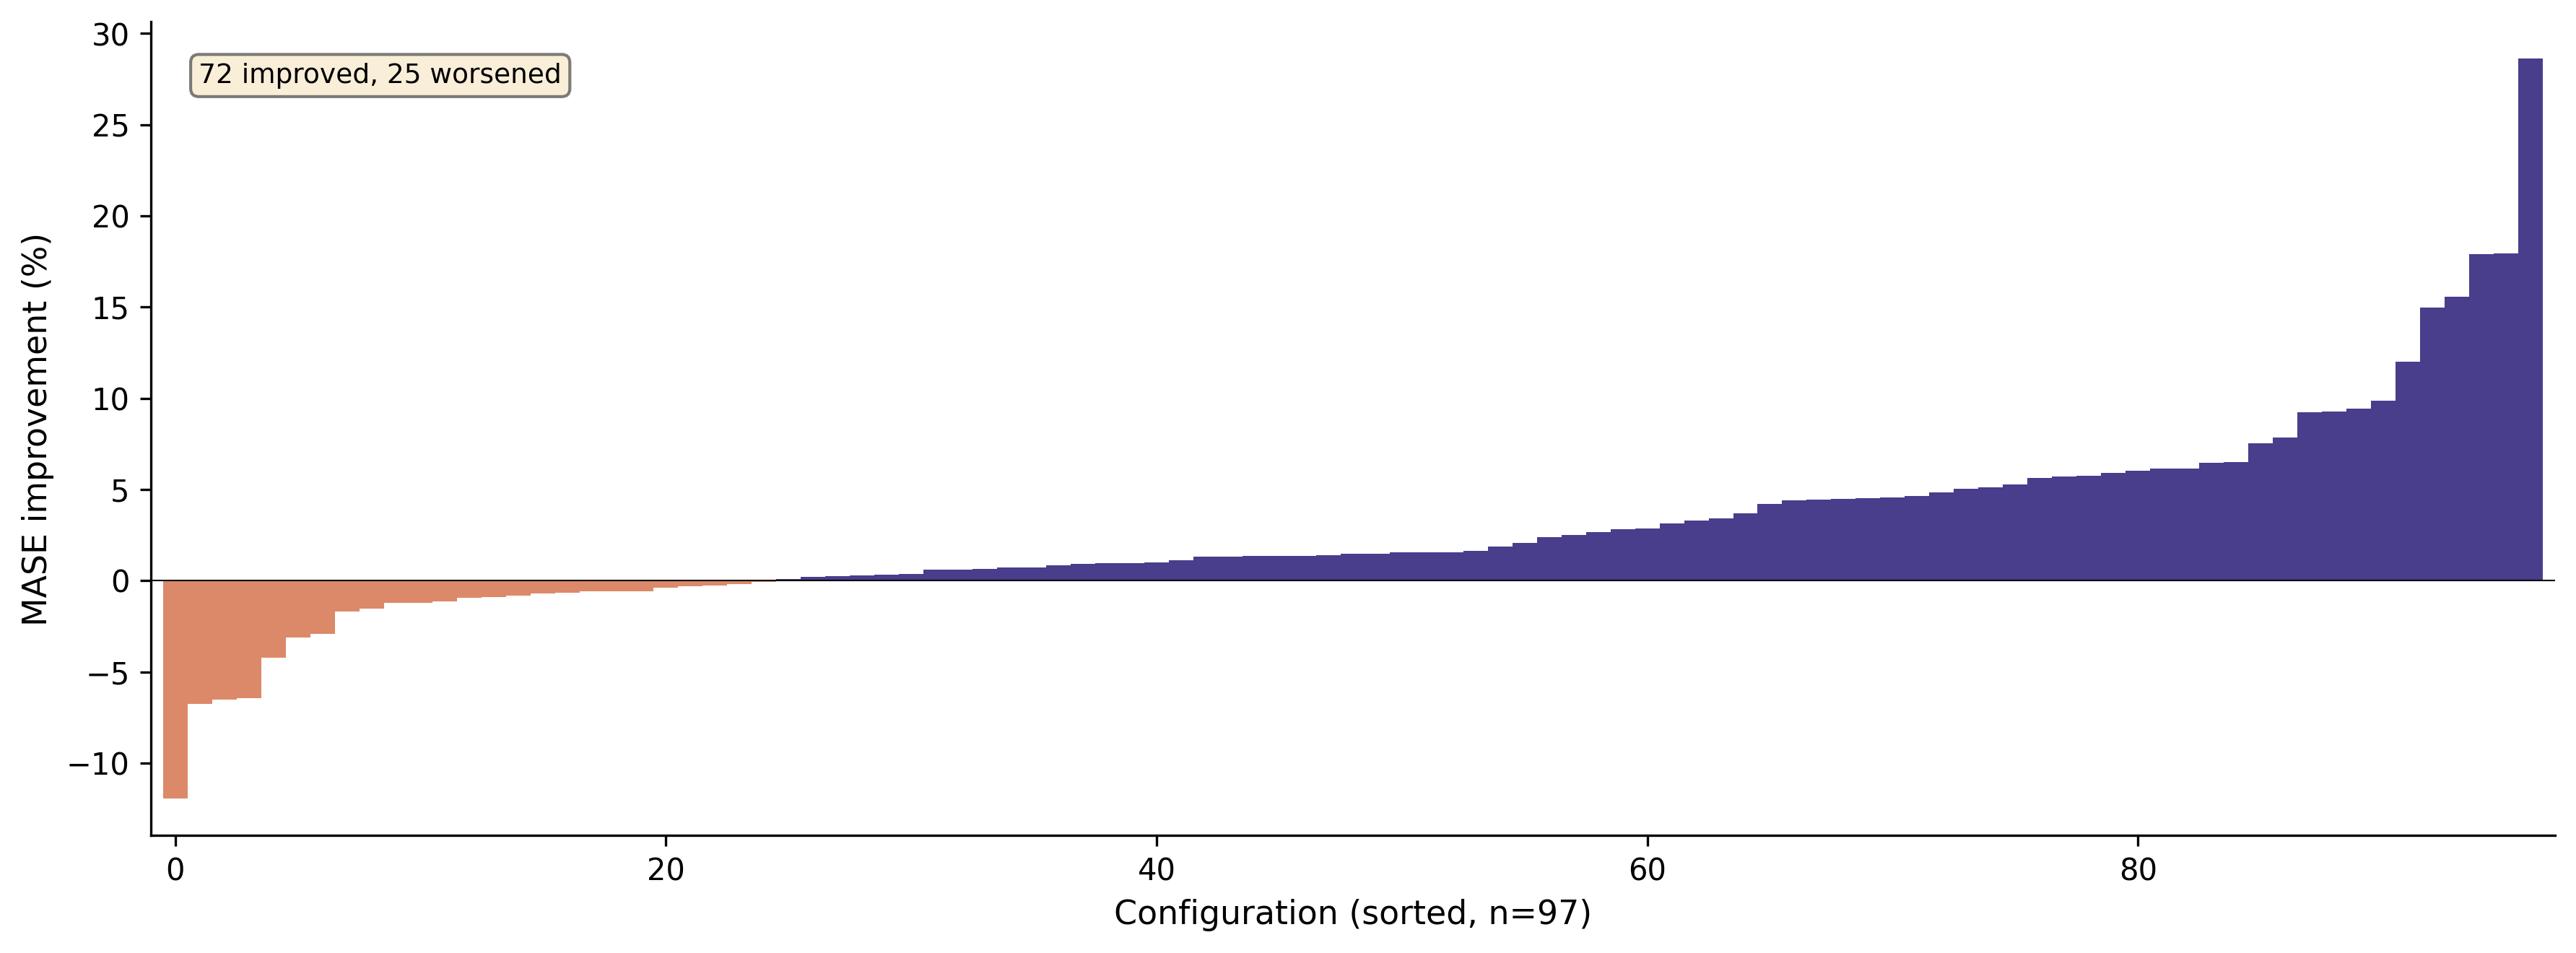
\includegraphics[width=\linewidth]{figures/fig_waterfall.pdf}
\caption{Per-configuration improvement (5-seed average), sorted. Green: HD10 wins. Red: baseline wins. 72/97 configurations improve.}
\label{fig:waterfall}
\end{figure}

\begin{figure}[t]
\centering
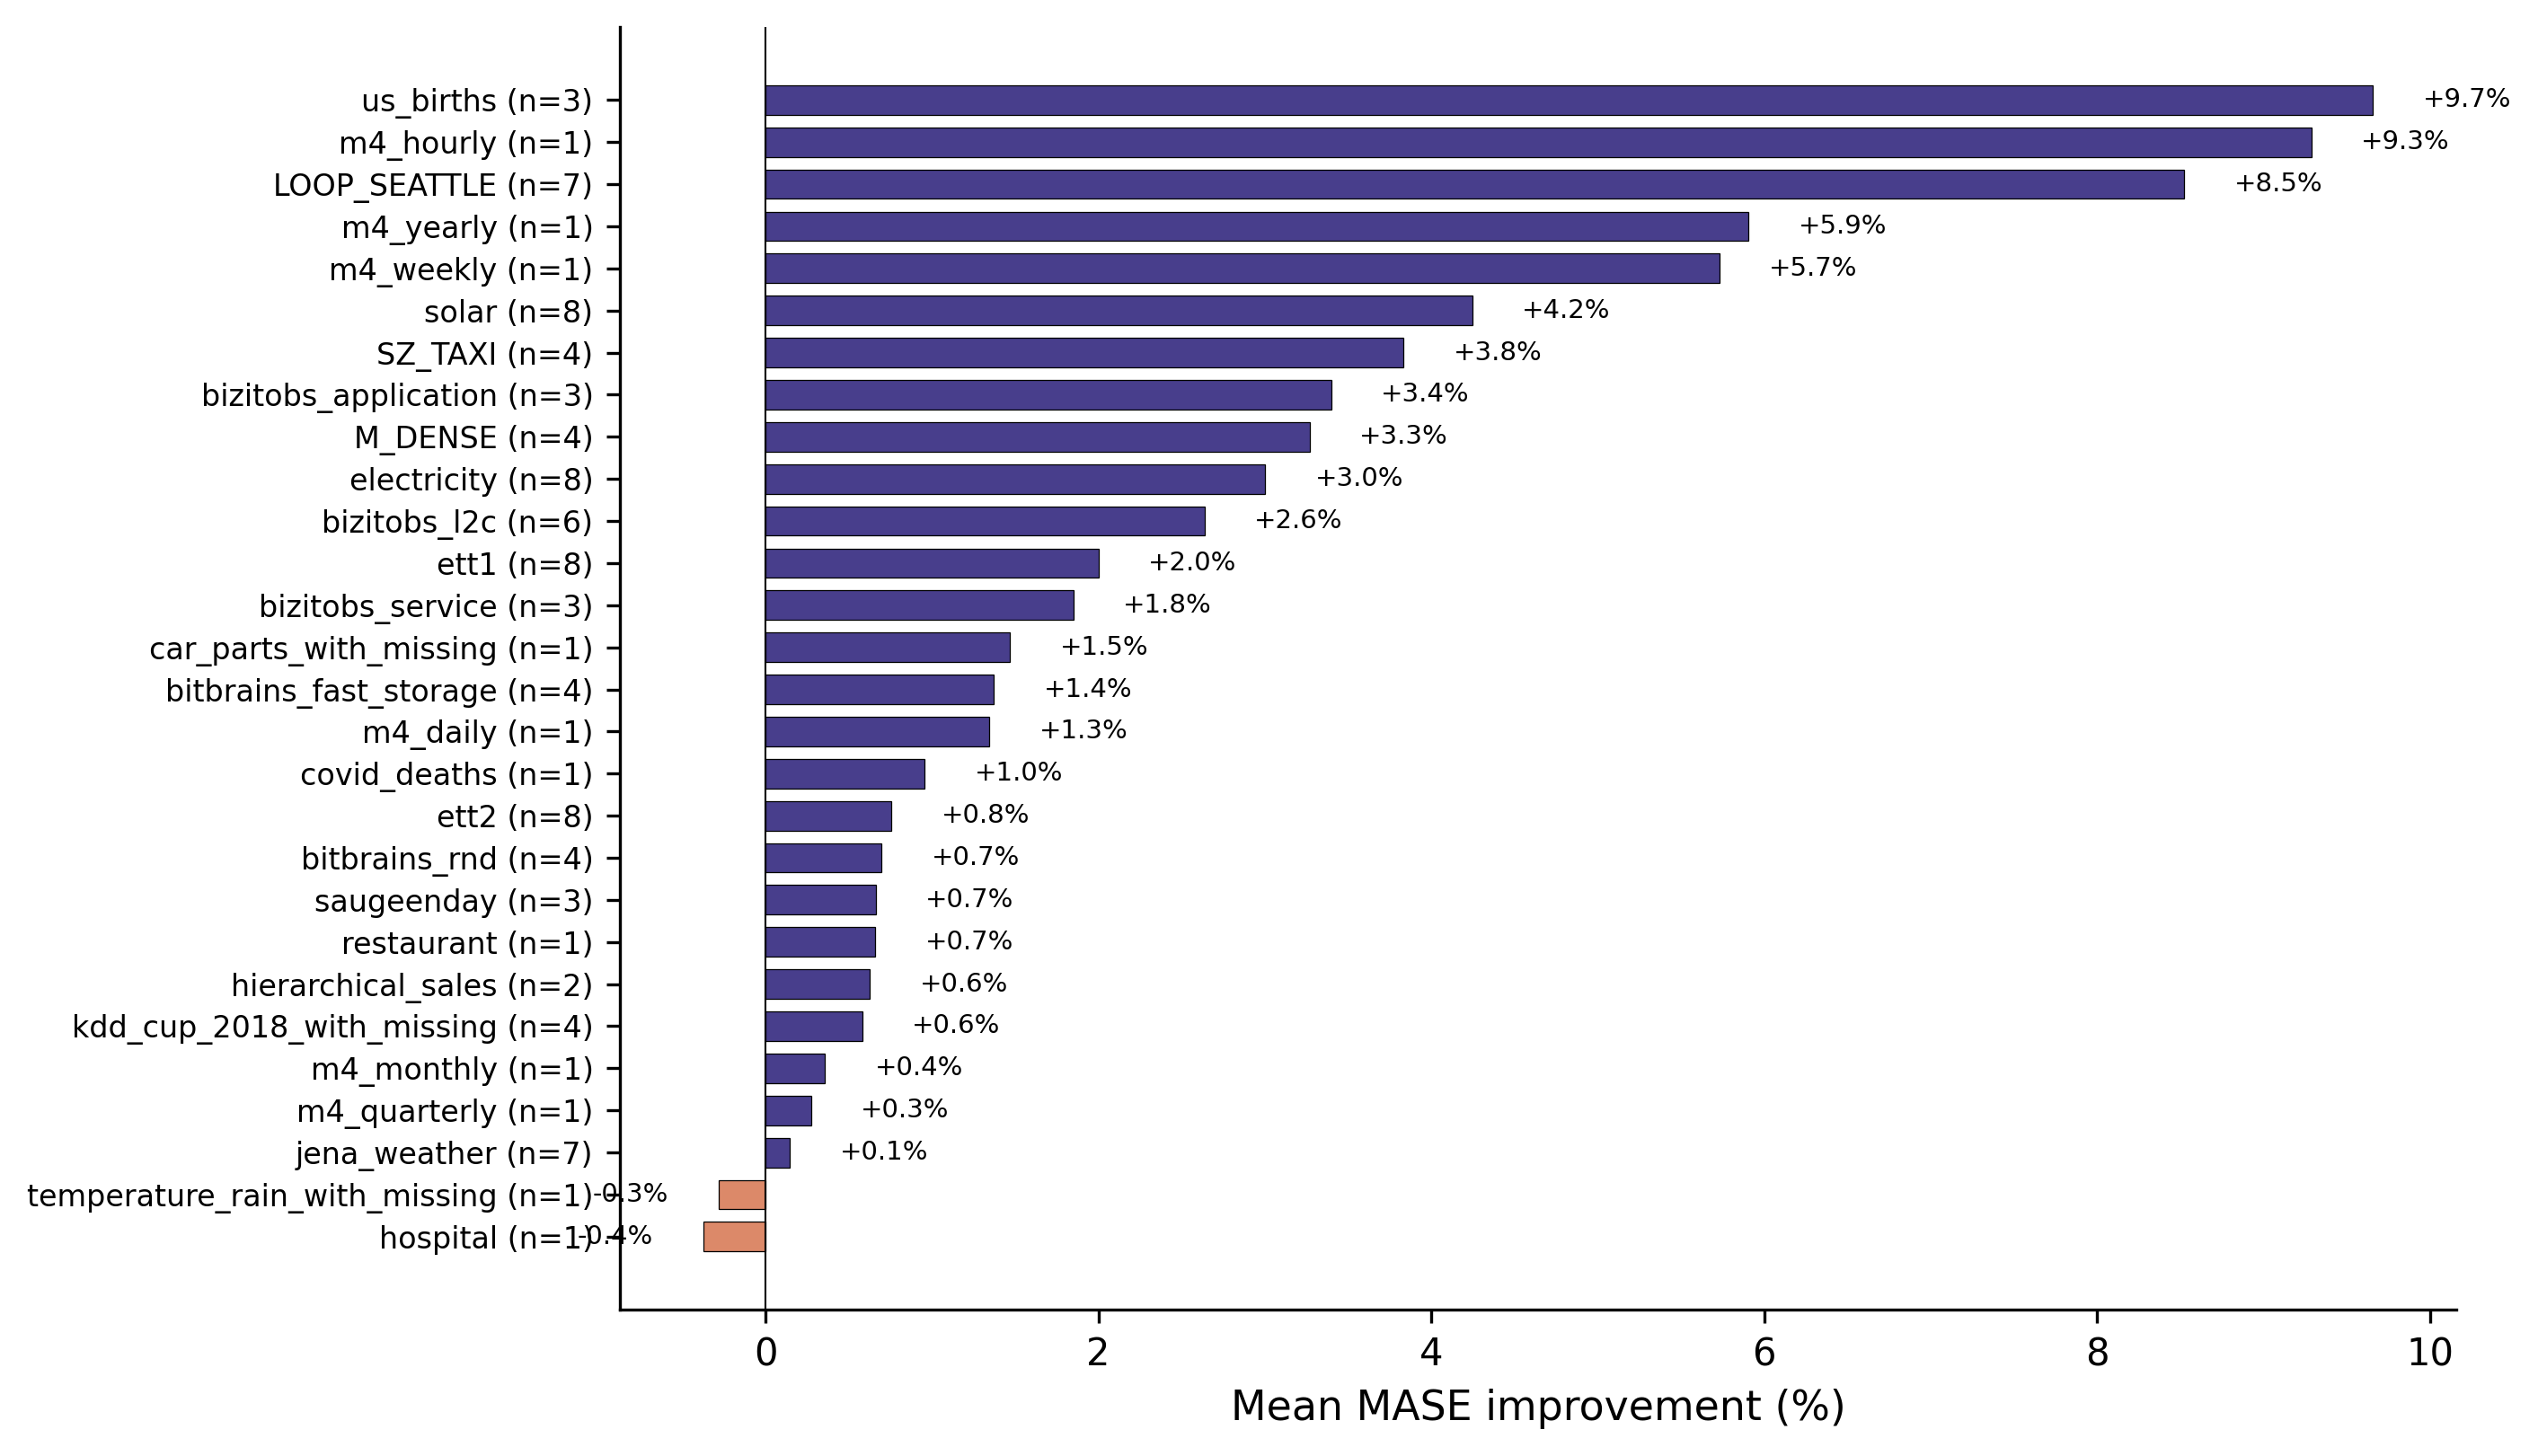
\includegraphics[width=\linewidth]{figures/fig_per_dataset.pdf}
\caption{Improvement by dataset (5-seed average). Parentheses show (improved/total) configurations. Transport and energy datasets benefit most; weather is neutral.}
\label{fig:perdataset}
\end{figure}

\subsection{Context length}

\begin{figure}[t]
\centering
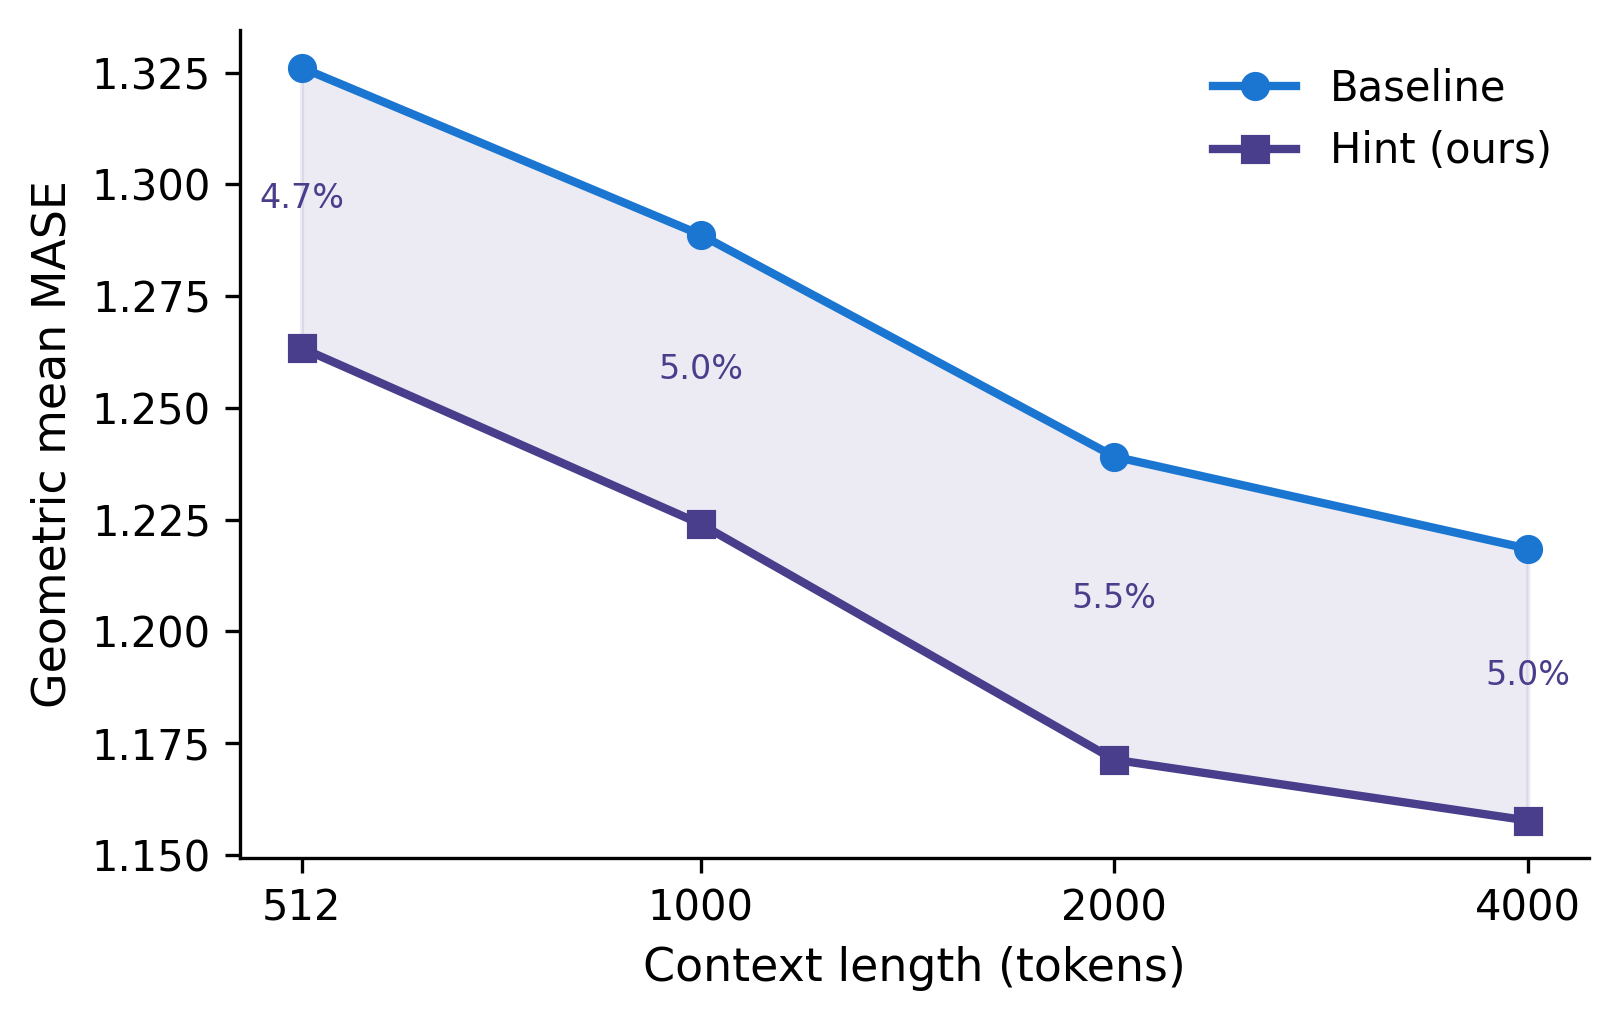
\includegraphics[width=0.55\linewidth]{figures/fig6_context_length.pdf}
\caption{The improvement from hint preconditioning is approximately constant ($\sim$5\%) across context lengths from 512 to 4,000.}
\label{fig:context}
\end{figure}

Figure~\ref{fig:context} shows that the benefit is approximately constant ($\sim$5\%) across context lengths from 512 to 4,000. Notably, HD10 at context length 2,000 (MASE 1.1713) outperforms the baseline at context length 4,000 (MASE 1.2185), suggesting that hint preconditioning can substitute for doubling the context window.

%==============================================================================
\section{Analysis}
%==============================================================================

\subsection{Mechanism}

The hint channel operates by providing each patch embedding with information about \emph{neighboring patches} at the input level, before any attention computation. For the Chebyshev $d=4$ filter with stride $s=16$:
\[
\tilde{h}[t] = h[t] - x[t] = -2 x[t-32] + 0.5 x[t-64],
\]
i.e., the hint residual for patch $i$ contains a weighted combination of values from patches $i-2$ and $i-4$. This injects cross-patch temporal information directly into the input embedding, reducing the burden on self-attention to discover these relationships.

The effectiveness of stride $s = P$ (patch-aligned lookback) supports this interpretation: when $s = P$, the filter taps land exactly on corresponding positions in neighboring patches, providing the most informative cross-patch signal. Misaligned strides ($s \neq P$) dilute this signal.

\subsection{Learning rate}
\label{sec:lr}

The hint channel interacts with the learning rate in an interesting way. Table~\ref{tab:lr_landscape} summarizes the full LR $\times$ method landscape.

\begin{table}[h]
\centering
\caption{Learning rate $\times$ method interaction (5-seed mean MASE).}
\label{tab:lr_landscape}
\small
\begin{tabular}{lccc}
\toprule
& $\eta = 10^{-3}$ & $\eta = 2 \times 10^{-3}$ & LR sensitivity \\
\midrule
Baseline & 1.2116 & 1.1841 & 2.27\% \\
HD10 (Ours) & 1.1765 & 1.1755 & 0.09\% \\
\midrule
HD10 vs BL & $-2.89\%$ $(p < 10^{-15})$ & $-0.72\%$ $(p = 3.8 \times 10^{-4})$ & \\
\bottomrule
\end{tabular}
\end{table}

Two effects are at play: (1) the baseline is \emph{undertrained} at $\eta = 10^{-3}$, and a higher learning rate closes most of the gap; (2) HD10 provides a genuine but smaller ($+0.72\%$) improvement even at matched optimal LR. We interpret this as the hint channel providing two distinct benefits:
\begin{itemize}
    \item \textbf{Optimization robustness}: HD10 achieves near-identical performance ($\sim$1.176) regardless of whether $\eta = 10^{-3}$ or $2 \times 10^{-3}$. The polynomial structure in the hint channel acts as an implicit regularizer that makes the optimization landscape more forgiving.
    \item \textbf{Genuine inductive bias}: At matched optimal LR, the polynomial content still provides a statistically significant 0.72\% improvement ($p = 3.8 \times 10^{-4}$, 280/485 wins). This residual benefit is attributable to the cross-patch information content of the Chebyshev filter.
\end{itemize}

The capacity controls (Section 5.1) are unaffected by this learning rate interaction, since all four conditions (Baseline, Zero, Duplicate, HD10) use the same $\eta = 10^{-3}$. Matched-LR capacity controls ($\eta = 2 \times 10^{-3}$) are in progress.

\subsection{Variance reduction}

Across 5 seeds and 97 configurations, HD10 reduces per-configuration coefficient of variation by 10.7\% relative to the baseline, with lower variance in 66\% of configurations. The correlation between baseline variance and HD10 improvement is $r = -0.66$: configurations with high seed-to-seed variance in the baseline benefit most from hint preconditioning ($-6.61\%$ improvement for the highest-variance quartile vs.\ $-0.40\%$ for the lowest). This suggests that hints act as a regularizer specifically targeting configurations where the model is most unstable.

%==============================================================================
\section{Limitations}
%==============================================================================

\begin{enumerate}
    \item \textbf{Learning rate interaction.} As discussed in Section~\ref{sec:lr}, the improvement at $\text{LR}=10^{-3}$ ($-2.89\%$) is substantially larger than at matched optimal LR ($-0.72\%$). The dominant effect is optimization robustness rather than pure inductive bias. The matched-LR benefit, while statistically significant ($p = 3.8 \times 10^{-4}$), is modest.
    \item \textbf{Domain heterogeneity.} The method provides no significant improvement on weather and healthcare datasets. These domains have temporal patterns at scales that do not align well with the filter's lookback distance.
    \item \textbf{Single model scale.} Our experiments use Moirai-2 Small (11.4M parameters). Preliminary experiments on the Base model (46M parameters) show inconsistent results across seeds, suggesting that larger models may not benefit from hint preconditioning, as the additional capacity is redundant when the model is sufficiently large.
    \item \textbf{Fixed filter coefficients.} Our filter uses fixed Chebyshev coefficients. Experiments with learned FIR coefficients show competitive results (Chebyshev-initialized: $-3.85\%$, zero-initialized: $-3.57\%$), but fixed Chebyshev remains slightly better, suggesting that the polynomial structure is close to optimal for this task.
\end{enumerate}

%==============================================================================
\section{Conclusion}
%==============================================================================

We have shown that a simple, fixed polynomial FIR filter applied as an auxiliary input channel to a patch-based time series transformer provides a statistically significant and robust improvement in forecasting accuracy. The method adds negligible overhead (0.11\% parameters, $\sim$1.6\% compute) and requires no modification to the transformer architecture itself. Through controlled ablations with duplicate and zero channels, we demonstrate that the improvement is driven by the polynomial content of the hint channel, not by extra capacity. The benefit is strongest for high-frequency domains and long prediction horizons, consistent with the mechanism of cross-patch information leakage at the filter's lookback scale.

Our work provides empirical evidence for the practical value of polynomial basis transformations in neural sequence models, connecting the theoretical framework of universal sequence preconditioning~\citep{marsden2024universal} to the applied setting of time series forecasting.

\bibliography{references}
\bibliographystyle{plainnat}

%==============================================================================
\appendix
\section{Detailed Experimental Methodology}
\label{app:methodology}
%==============================================================================

\subsection{Training Protocol}

All experiments use identical training infrastructure on NVIDIA H100/A100 GPUs via SLURM on the Princeton PLI/Della cluster. The complete training configuration:

\begin{center}
\small
\begin{tabular}{ll}
\toprule
\textbf{Parameter} & \textbf{Value} \\
\midrule
Architecture & Moirai-2 Small (6 layers, $d=384$, $d_{\text{ff}}=1024$, $P=16$) \\
Total parameters & 11.4M (baseline), 11.4M + 12K (HD10) \\
Training data & LOTSA v1, Moirai-2 config (weighted, variate-proportional) \\
Steps (10K runs) & 100 epochs $\times$ 100 batches = 10,000 steps \\
Steps (100K runs) & 1,000 epochs $\times$ 100 batches = 100,000 steps \\
Batch size & 256 \\
Optimizer & AdamW ($\beta_1=0.9$, $\beta_2=0.98$, $\epsilon=10^{-6}$, wd $=0.1$) \\
LR schedule & Cosine annealing, peak $\eta = 10^{-3}$, min $\eta = 0$ \\
Warmup & 1,000 steps (linear) \\
Precision & bf16 mixed precision \\
Anomaly filtering & $z$-score threshold = 8.0, variance ratio = 0.0 (disabled) \\
Random seeds & 0, 1, 2, 7, 42 (5 seeds for main results) \\
\bottomrule
\end{tabular}
\end{center}

\subsection{Evaluation Protocol}

All evaluations use the GIFT-Eval benchmark~\citep{vijay2024gifteval} with 97 dataset$\times$horizon configurations:
\begin{itemize}
    \item Context length: 4,000 tokens (maximum supported)
    \item Patch size: 32 for most frequencies, 8 for quarterly (following Moirai conventions)
    \item Batch size: 64
    \item Metric: MASE (Mean Absolute Scaled Error) per configuration
    \item Aggregation: geometric mean across 97 configurations
    \item Statistical test: paired sign test (binomial test, two-sided) on per-configuration wins
    \item Pooling: across seeds, giving $5 \times 97 = 485$ comparisons
\end{itemize}

\subsection{Hint Channel Implementation}

The Chebyshev polynomial $T_d(z)$ is expanded in the monomial basis to obtain FIR filter coefficients $c_0, \ldots, c_d$. The hint signal for time step $t$ is:
\[
\tilde{h}[t] = \left(\sum_{k=0}^{d} c_k \, x[t - ks]\right) - x[t]
\]
This is computed over the full (normalized, zero-mean unit-variance) time series before patching. Unobserved time steps are masked to zero. During training with hint dropout $p$, each patch's hint independently has probability $p$ of being replaced with zeros. At inference, the full hint is always provided.

The hint channel is concatenated with the target and mask channels before the input projection:
\[
\mathbf{e}_i = \text{ResBlock}_{(2+n_h)P \to d}([\mathbf{p}_i; \mathbf{m}_i; \tilde{\mathbf{h}}^{(1)}_i; \ldots; \tilde{\mathbf{h}}^{(n_h)}_i])
\]
where $n_h = 1$ for single-scale (HD10) and $n_h = 2$ for multi-scale (MSHD10). The ResBlock consists of:
\begin{align}
\mathbf{z} &= \text{SiLU}(W_1 \mathbf{x} + b_1) & W_1 &\in \mathbb{R}^{d \times (2+n_h)P} \\
\mathbf{o} &= W_2 \mathbf{z} + b_2 + W_3 \mathbf{x} + b_3 & W_2 &\in \mathbb{R}^{d \times d}, \; W_3 \in \mathbb{R}^{d \times (2+n_h)P}
\end{align}
Only $W_1$ and $W_3$ are wider than the baseline. $W_2$ and all downstream layers are identical.

%==============================================================================
\section{Per-Seed Detailed Results}
\label{app:seeds}
%==============================================================================

\begin{table}[h]
\centering
\caption{HD10 vs.\ Baseline: per-seed pairwise comparison (10K steps, $\eta = 10^{-3}$).}
\small
\begin{tabular}{cccccc}
\toprule
\textbf{Seed} & \textbf{BL MASE} & \textbf{HD10 MASE} & \textbf{$\Delta$\%} & \textbf{Wins/97} & \textbf{$p$-value} \\
\midrule
0 & 1.2185 & 1.1577 & $+4.99\%$ & 66 & $2.5 \times 10^{-4}$ \\
1 & 1.1955 & 1.1902 & $+0.44\%$ & 54 & 0.155 \\
2 & 1.2134 & 1.1798 & $+2.77\%$ & 70 & $7.4 \times 10^{-6}$ \\
7 & 1.2198 & 1.1698 & $+4.11\%$ & 78 & $5.8 \times 10^{-10}$ \\
42 & 1.2111 & 1.1852 & $+2.13\%$ & 61 & $7.2 \times 10^{-3}$ \\
\midrule
\textbf{Pooled} & & & \textbf{$+2.89\%$} & \textbf{329/485} & $\mathbf{1.5 \times 10^{-15}}$ \\
\bottomrule
\end{tabular}
\end{table}

\begin{figure}[h]
\centering
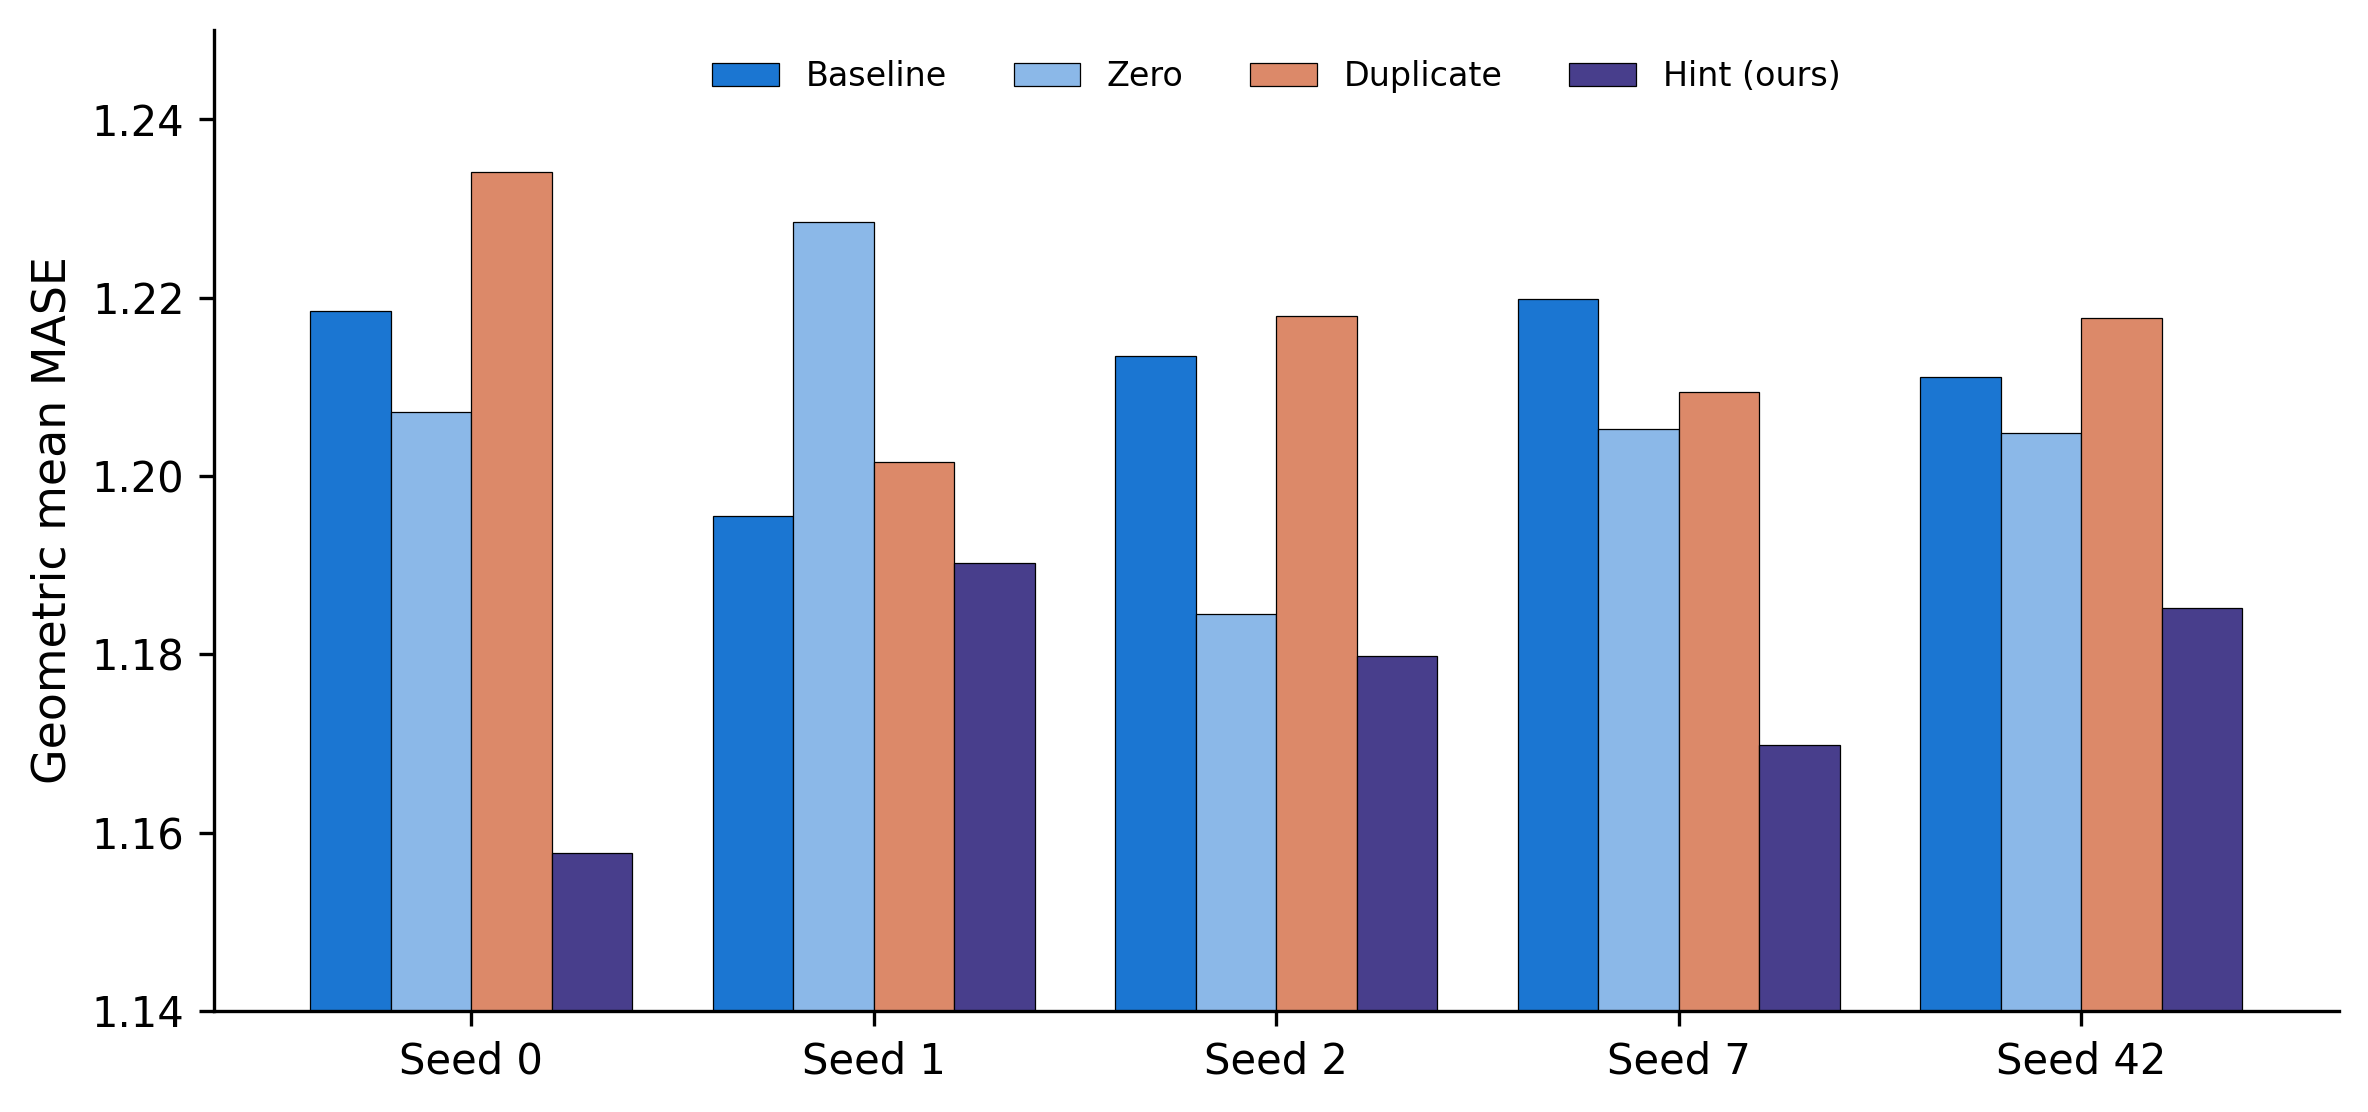
\includegraphics[width=0.85\linewidth]{figures/fig5_seed_robustness.pdf}
\caption{Per-seed MASE for all four conditions. HD10 (green) achieves the lowest MASE on every seed.}
\label{fig:seeds}
\end{figure}

When averaging each configuration's MASE across all 5 seeds, HD10 wins 72/97 configurations ($p_{\text{sign}} = 9.6 \times 10^{-7}$; $p_{\text{Wilcoxon}} = 9.0 \times 10^{-9}$; $p_{t\text{-test}} = 2.4 \times 10^{-6}$). HD10 wins 3+ out of 5 seeds on 76.3\% of configurations, and wins all 5 seeds on 23 configurations. Only 2 configurations (bizitobs\_l2c/5T/medium, electricity/15T/short) see the baseline win all 5 seeds.

%==============================================================================
\section{Multi-Scale Variants}
\label{app:multiscale}
%==============================================================================

We test two multi-scale variants that provide two hint channels (degree 4 + degree 6):

\begin{table}[h]
\centering
\caption{Multi-scale variants (5 seeds, $\eta = 10^{-3}$, 10K steps).}
\small
\begin{tabular}{lcccccc}
\toprule
\textbf{Method} & \textbf{Mean} & \textbf{Std} & \textbf{vs BL} & \textbf{Wins/485} & \textbf{$p$} \\
\midrule
HD10 (d=4, 10\% drop) & 1.1765 & 0.0116 & $-2.89\%$ & 329 & $1.5 \times 10^{-15}$ \\
MS46 (d=4+6, 0\% drop) & 1.1858 & 0.0173 & $-2.13\%$ & 330 & $6.8 \times 10^{-16}$ \\
MSHD10 (d=4+6, 10\% drop) & 1.1863 & 0.0101 & $-2.09\%$ & 315 & $2.2 \times 10^{-11}$ \\
\bottomrule
\end{tabular}
\end{table}

All three methods are statistically indistinguishable head-to-head (HD10 vs MS46: 251/485, $p=0.47$; HD10 vs MSHD10: 257/485, $p=0.20$). MS46 is the only method where all 5/5 individual seeds are significant. MSHD10 has the lowest cross-seed standard deviation (0.0101 vs HD10's 0.0116).

%==============================================================================
\section{Complete Experiment Catalog}
\label{app:catalog}
%==============================================================================

We conducted 84 distinct training runs across the project. The following tables list all experiments with their configurations and results, organized by category. All results use geometric mean MASE on GIFT-Eval (97 configurations) at context length 4,000. ``Wins'' indicates configs where the method beats the matched-seed baseline. Boldface indicates the best in each category.

\subsection{Capacity Controls (5 seeds, $\eta = 10^{-3}$, 10K steps)}

\begin{table}[h]
\centering
\caption{Capacity control experiments. Same architecture width, different channel content.}
\label{tab:catalog_capacity}
\small
\begin{tabular}{lccccc}
\toprule
\textbf{Method} & \textbf{Content} & \textbf{Mean} & \textbf{Std} & \textbf{Wins/485} & \textbf{$p$} \\
\midrule
\textbf{HD10} & Chebyshev $T_4(B^{16})$ & \textbf{1.1765} & 0.0116 & \textbf{329} & $1.5 \times 10^{-15}$ \\
Zero & All zeros & 1.2061 & 0.0143 & 262 & 0.042 \\
Baseline & No extra channel & 1.2116 & 0.0087 & --- & --- \\
Duplicate & Copy of input & 1.2162 & 0.0114 & 217 & 0.99 \\
\bottomrule
\end{tabular}
\end{table}

\subsection{Polynomial Degree (seed 0, Chebyshev, $s=16$, 10\% dropout)}

\begin{table}[h]
\centering
\small
\begin{tabular}{ccccc}
\toprule
\textbf{Degree} & \textbf{Effective lags} & \textbf{MASE} & \textbf{$\Delta$\% vs BL} & \textbf{Wins/97} \\
\midrule
\textbf{4} & 2 (at $2P$, $4P$) & \textbf{1.1577} & $-4.99\%$ & \textbf{66} \\
2 & 1 (at $2P$) & 1.1794 & $-3.20\%$ & 63 \\
6 & 3 (at $2P$, $4P$, $6P$) & 1.1733 & $-3.71\%$ & 69 \\
8 & 4 (at $2P$--$8P$) & 1.1828 & $-2.92\%$ & 62 \\
3 & 1 (at $3P$) & 1.1947 & $-1.95\%$ & 55 \\
0 (dup) & 0 & 1.2068 & $-0.96\%$ & 42 \\
\bottomrule
\end{tabular}
\end{table}

\subsection{Filter Stride (seed 0, Chebyshev $d=4$, 10\% dropout)}

\begin{table}[h]
\centering
\small
\begin{tabular}{ccccc}
\toprule
\textbf{Stride} & \textbf{Lookback} & \textbf{MASE} & \textbf{$\Delta$\% vs BL} & \textbf{Wins/97} \\
\midrule
\textbf{16 ($=P$)} & 32, 64 steps & \textbf{1.1577} & $-4.99\%$ & \textbf{66} \\
4 & 8, 16 steps & 1.1819 & $-3.00\%$ & 57 \\
8 & 16, 32 steps & 1.1977 & $-1.71\%$ & 62 \\
32 & 64, 128 steps & 1.1929 & $-2.10\%$ & 63 \\
8+16 (dual) & 16, 32, 64 steps & 1.1795 & $-3.20\%$ & 62 \\
\bottomrule
\end{tabular}
\end{table}

\subsection{Filter Basis (seed 0, $d=4$, $s=16$, 10\% dropout)}

\begin{table}[h]
\centering
\small
\begin{tabular}{lcccccc}
\toprule
\textbf{Basis} & \textbf{MASE} & \textbf{$\Delta$\%} & \textbf{Wins vs BL} & \textbf{$p$} & \textbf{vs Cheby} & \textbf{$p$} \\
\midrule
\textbf{Chebyshev} & \textbf{1.1577} & $-4.99\%$ & 66/97 & $2.5 \times 10^{-4}$ & --- & --- \\
EMA & 1.1711 & $-3.89\%$ & 65/97 & $5.3 \times 10^{-4}$ & 41/97 & 0.077 \\
Legendre $d=4$ & 1.1810 & $-3.07\%$ & 62/97 & $4.0 \times 10^{-3}$ & 30/97 & $<$0.001 \\
Legendre $d=6$ & 1.1806 & $-3.10\%$ & 64/97 & $1.1 \times 10^{-3}$ & 50/97 & 0.42 \\
Finite Diff & 1.2048 & $-1.12\%$ & 54/97 & 0.16 & 29/97 & $<$0.001 \\
Duplicate & 1.2068 & $-0.96\%$ & 42/97 & 0.11 & 27/97 & $<$0.001 \\
\bottomrule
\end{tabular}
\end{table}

\subsection{Hint Dropout Rate (seed 0, Chebyshev $d=4$, $s=16$)}

\begin{table}[h]
\centering
\small
\begin{tabular}{ccccc}
\toprule
\textbf{Dropout} & \textbf{MASE} & \textbf{$\Delta$\% vs BL} & \textbf{Wins/97} & \textbf{$p$} \\
\midrule
0\% (HD0) & \multicolumn{4}{c}{\emph{pending (submitted)}} \\
2\% & 1.1794 & $-3.20\%$ & 63 & 0.004 \\
3\% & 1.1947 & $-1.95\%$ & 55 & 0.22 \\
\textbf{10\%} & \textbf{1.1577} & $\mathbf{-4.99\%}$ & \textbf{66} & \textbf{0.0005} \\
20\% & 1.1842 & $-2.81\%$ & 67 & 0.0002 \\
30\% & 1.2034 & $-1.23\%$ & 61 & 0.014 \\
\bottomrule
\end{tabular}
\end{table}

\subsection{Inference-Time Content Ablation (seed 0, HD10 model)}

A model trained with Chebyshev hints is evaluated with different hint content at inference:

\begin{table}[h]
\centering
\small
\begin{tabular}{lcc}
\toprule
\textbf{Inference hint content} & \textbf{MASE} & \textbf{vs Normal} \\
\midrule
Normal (Chebyshev) & 1.1577 & --- \\
No hint channel (Baseline arch) & 1.2185 & $+5.2\%$ \\
Zeros & 1.2658 & $+9.3\%$ \\
Random Gaussian noise & 1.3254 & $+14.5\%$ \\
Duplicate (copy of input) & 1.5043 & $+29.9\%$ \\
\bottomrule
\end{tabular}
\end{table}

\subsection{Learned FIR Coefficients (seed 0)}

Instead of fixed Chebyshev coefficients, the filter weights are made learnable:

\begin{table}[h]
\centering
\small
\begin{tabular}{lccc}
\toprule
\textbf{Initialization} & \textbf{Learned coefficients} & \textbf{MASE} & \textbf{$\Delta$\% vs BL} \\
\midrule
Chebyshev init & $[-0.026, -1.032, -0.123, 0.007]$ & 1.1715 & $-3.85\%$ \\
Zero init & $[0.308, 0.177, 0.057, 0.045]$ & 1.1751 & $-3.57\%$ \\
Fixed Chebyshev & $[0, -2, 0, 0.5]$ (not learned) & 1.1577 & $-4.99\%$ \\
\bottomrule
\end{tabular}
\end{table}

The two learned filters converge to distinct basins (high-pass vs.\ smoothing). Both beat the baseline significantly but are slightly worse than the fixed Chebyshev (51/97 h2h, $p=0.34$).

\subsection{Latent Preconditioning (seed 0)}

Applying the polynomial filter \emph{after} the input projection (in latent space) rather than before patching:

\begin{table}[h]
\centering
\small
\begin{tabular}{lccc}
\toprule
\textbf{Method} & \textbf{Filter location} & \textbf{MASE} & \textbf{vs BL} \\
\midrule
HD10 (input-level) & Before patching & 1.1577 & $-4.99\%$ \\
Latent $s=1$ & After input projection & 1.6223 & $+33.1\%$ \\
Latent $s=4$ & After input projection & 1.7214 & $+41.3\%$ \\
\bottomrule
\end{tabular}
\end{table}

Latent preconditioning is catastrophic. The filter must operate on the raw time series, not on learned embeddings.

\subsection{Context Length (seed 0)}

\begin{table}[h]
\centering
\small
\begin{tabular}{ccccc}
\toprule
\textbf{Context} & \textbf{BL} & \textbf{HD10} & \textbf{$\Delta$\%} & \textbf{Wins/97} \\
\midrule
512 & 1.3261 & 1.2634 & $-4.73\%$ & 62 \\
1,000 & 1.2887 & 1.2240 & $-5.02\%$ & 65 \\
2,000 & 1.2391 & 1.1713 & $-5.47\%$ & 71 \\
4,000 & 1.2185 & 1.1577 & $-4.99\%$ & 66 \\
\bottomrule
\end{tabular}
\end{table}

\subsection{100K Training (3 seeds)}

\begin{table}[h]
\centering
\caption{Results at the full 100K training budget (3 seeds).}
\small
\begin{tabular}{lcccc}
\toprule
& \textbf{Seed 0} & \textbf{Seed 2} & \textbf{Seed 7} & \textbf{Mean} \\
\midrule
Baseline & 1.2783 & 1.2138 & 1.2149 & 1.2357 \\
HD10 & 1.1739 & 1.2072 & 1.1880 & 1.1897 \\
MSHD10 & 1.1622 & 1.1856 & 1.1862 & 1.1780 \\
\midrule
HD10 $\Delta$\% & $-8.17\%$ & $-0.54\%$ & $-2.21\%$ & $-3.72\%$ \\
MSHD10 $\Delta$\% & $-9.08\%$ & $-2.32\%$ & $-2.36\%$ & $-4.67\%$ \\
\bottomrule
\end{tabular}
\end{table}

Note: Baseline seed 0 exhibits training instability at 80K steps (MASE spikes to 1.3038 before partial recovery to 1.2783). Seeds 2 and 7 do not exhibit this behavior. This instability is likely related to the cosine learning rate schedule approaching zero; control experiments with cosine-floor and WSD schedules are in progress.

\subsection{Matched Learning Rate (5 seeds, $\eta = 2 \times 10^{-3}$)}

\begin{table}[h]
\centering
\caption{BL and HD10 at matched learning rate $\eta = 2 \times 10^{-3}$.}
\small
\begin{tabular}{cccccc}
\toprule
\textbf{Seed} & \textbf{BL@2e-3} & \textbf{HD10@2e-3} & \textbf{$\Delta$\%} & \textbf{Wins/97} & \textbf{$p$-value} \\
\midrule
0 & 1.1844 & 1.1725 & $+1.01\%$ & 57 & 0.052 \\
1 & 1.1869 & 1.1723 & $+1.23\%$ & 55 & 0.111 \\
2 & 1.1779 & 1.1906 & $-1.07\%$ & 46 & 0.729 \\
7 & 1.1724 & 1.1740 & $-0.13\%$ & 54 & 0.155 \\
42 & 1.1987 & 1.1680 & $+2.55\%$ & 68 & $4.7 \times 10^{-5}$ \\
\midrule
\textbf{Pooled} & \textbf{1.1841} & \textbf{1.1755} & $+0.72\%$ & \textbf{280/485} & $3.8 \times 10^{-4}$ \\
\bottomrule
\end{tabular}
\end{table}

\subsection{Base Model Scale (46M parameters, 10K steps)}

\begin{table}[h]
\centering
\small
\begin{tabular}{ccccc}
\toprule
\textbf{Seed} & \textbf{BL (46M)} & \textbf{HD10 (46M)} & \textbf{$\Delta$\%} & \textbf{Wins} \\
\midrule
0 & 1.1956 & 1.1979 & $-0.19\%$ & 52/95 \\
1 & 1.1913 & 1.1963 & $-0.42\%$ & 60/95 \\
42 & 1.2050 & 1.1834 & $+1.80\%$ & 59/93 \\
\bottomrule
\end{tabular}
\end{table}

Results are inconsistent at the 46M scale. The hint channel's benefit appears specific to capacity-constrained models.

\subsection{Prediction Horizon Effect (seed 0)}

\begin{table}[h]
\centering
\small
\begin{tabular}{ccc}
\toprule
\textbf{Prediction length} & \textbf{HD10 $\Delta$\%} & \textbf{Win rate} \\
\midrule
30 & $-0.1\%$ & 57\% \\
48 & $-2.1\%$ & 70\% \\
480 & $-6.7\%$ & 68\% \\
720 & $-8.6\%$ & 79\% \\
900 & $-14.1\%$ & 100\% \\
\bottomrule
\end{tabular}
\end{table}

\subsection{Model Soup (seed 0)}

Weight averaging between baseline and HD10 checkpoints:

\begin{table}[h]
\centering
\small
\begin{tabular}{lcc}
\toprule
\textbf{Method} & \textbf{MASE} \\
\midrule
Baseline & 1.2185 \\
HD10 & 1.1577 \\
Soup ($\alpha=0.5$) & 1.1680 \\
Soup ($\alpha=0.7$) & 1.1600 \\
\bottomrule
\end{tabular}
\end{table}

\subsection{Zero-Hint Dependence vs Dropout Rate (seed 0)}

Models trained with different hint dropout rates, evaluated with hint channel replaced by zeros:

\begin{table}[h]
\centering
\small
\begin{tabular}{ccccc}
\toprule
\textbf{Train dropout} & \textbf{Normal MASE} & \textbf{Zero-hint MASE} & \textbf{Degradation} \\
\midrule
0\% (MS46) & 1.1999 & 1.6301 & $+35.9\%$ \\
2\% & 1.1794 & 1.2648 & $+7.2\%$ \\
10\% (HD10) & 1.1577 & 1.2658 & $+9.3\%$ \\
30\% & 1.2034 & 1.2329 & $+2.5\%$ \\
\bottomrule
\end{tabular}
\end{table}

Without dropout, the model is catastrophically dependent on hints (36\% degradation when removed). With 10\% dropout, degradation is moderate (9\%), and with 30\% the model barely uses hints at all (2.5\% degradation but weaker overall performance).

\subsection{Computational Overhead}

Measured across 9 paired runs (HD10 and BL on the same GPU node):

\begin{table}[h]
\centering
\small
\begin{tabular}{lcc}
\toprule
& \textbf{Baseline} & \textbf{HD10} \\
\midrule
Training throughput & 2.18 it/s & 2.14 it/s ($-$1.6\%) \\
Extra parameters & 0 & 12,288 ($+$0.11\%) \\
Peak GPU memory & identical & identical \\
\bottomrule
\end{tabular}
\end{table}

\subsection{Seed Consistency Distribution}

\begin{figure}[h]
\centering
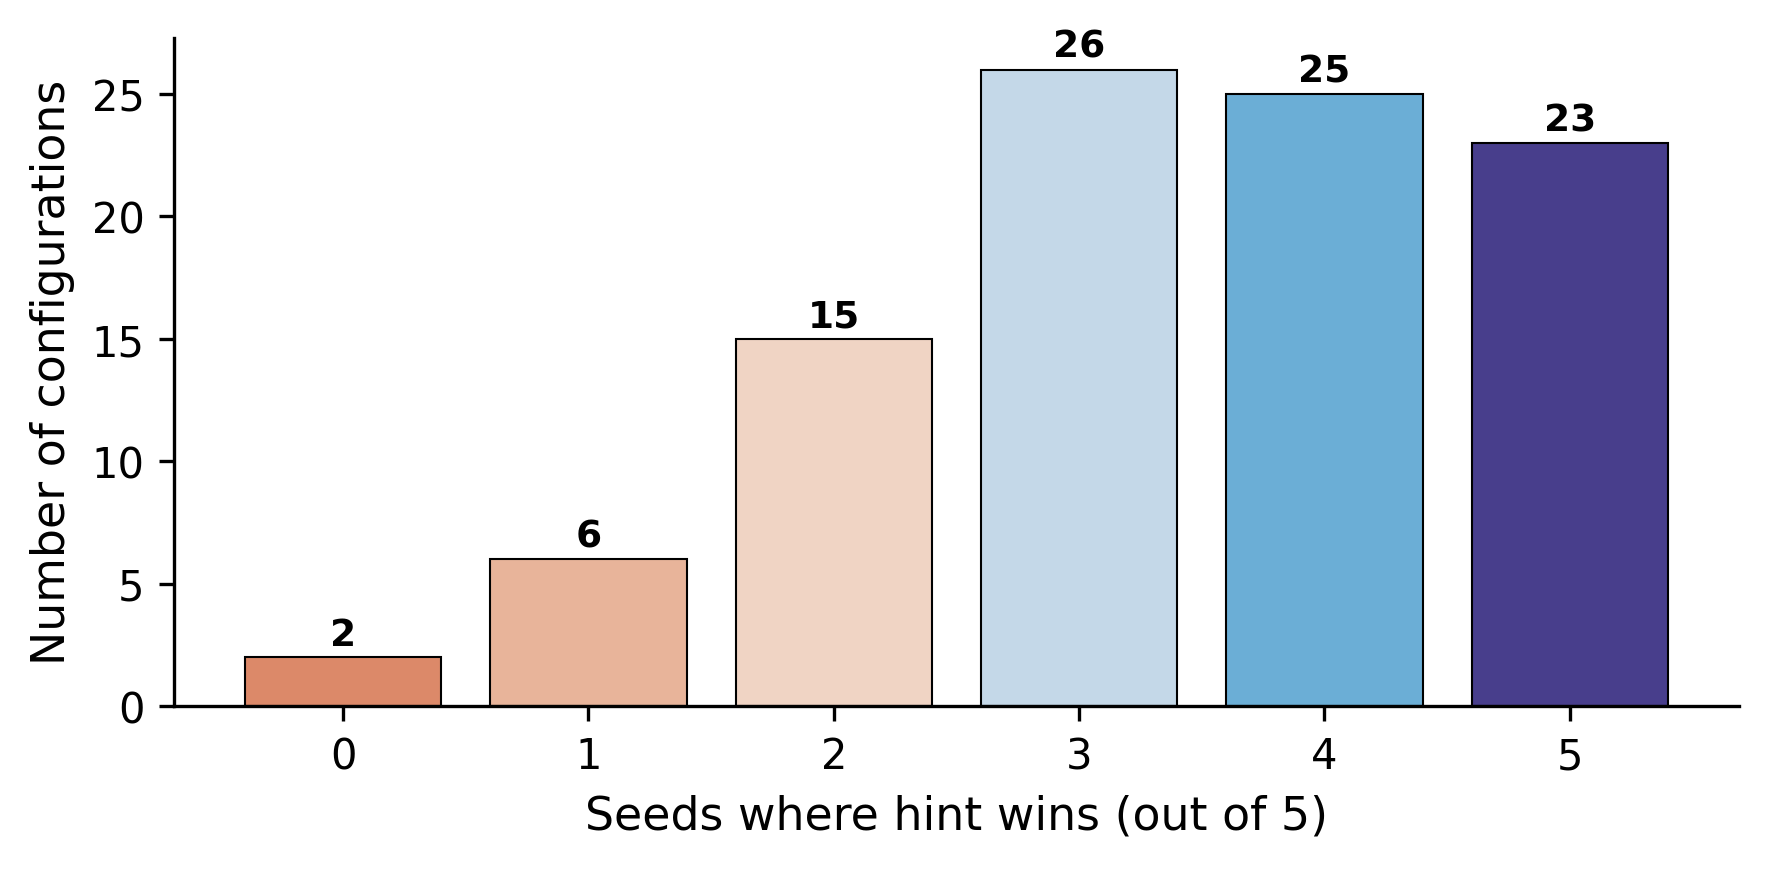
\includegraphics[width=0.6\linewidth]{figures/fig_seed_consistency.pdf}
\caption{For each configuration, how many of 5 seeds does HD10 win? 74 of 97 configs see HD10 win the majority ($\geq 3/5$) of seeds.}
\end{figure}

\subsection{Representative Configurations}

\begin{figure}[h]
\centering
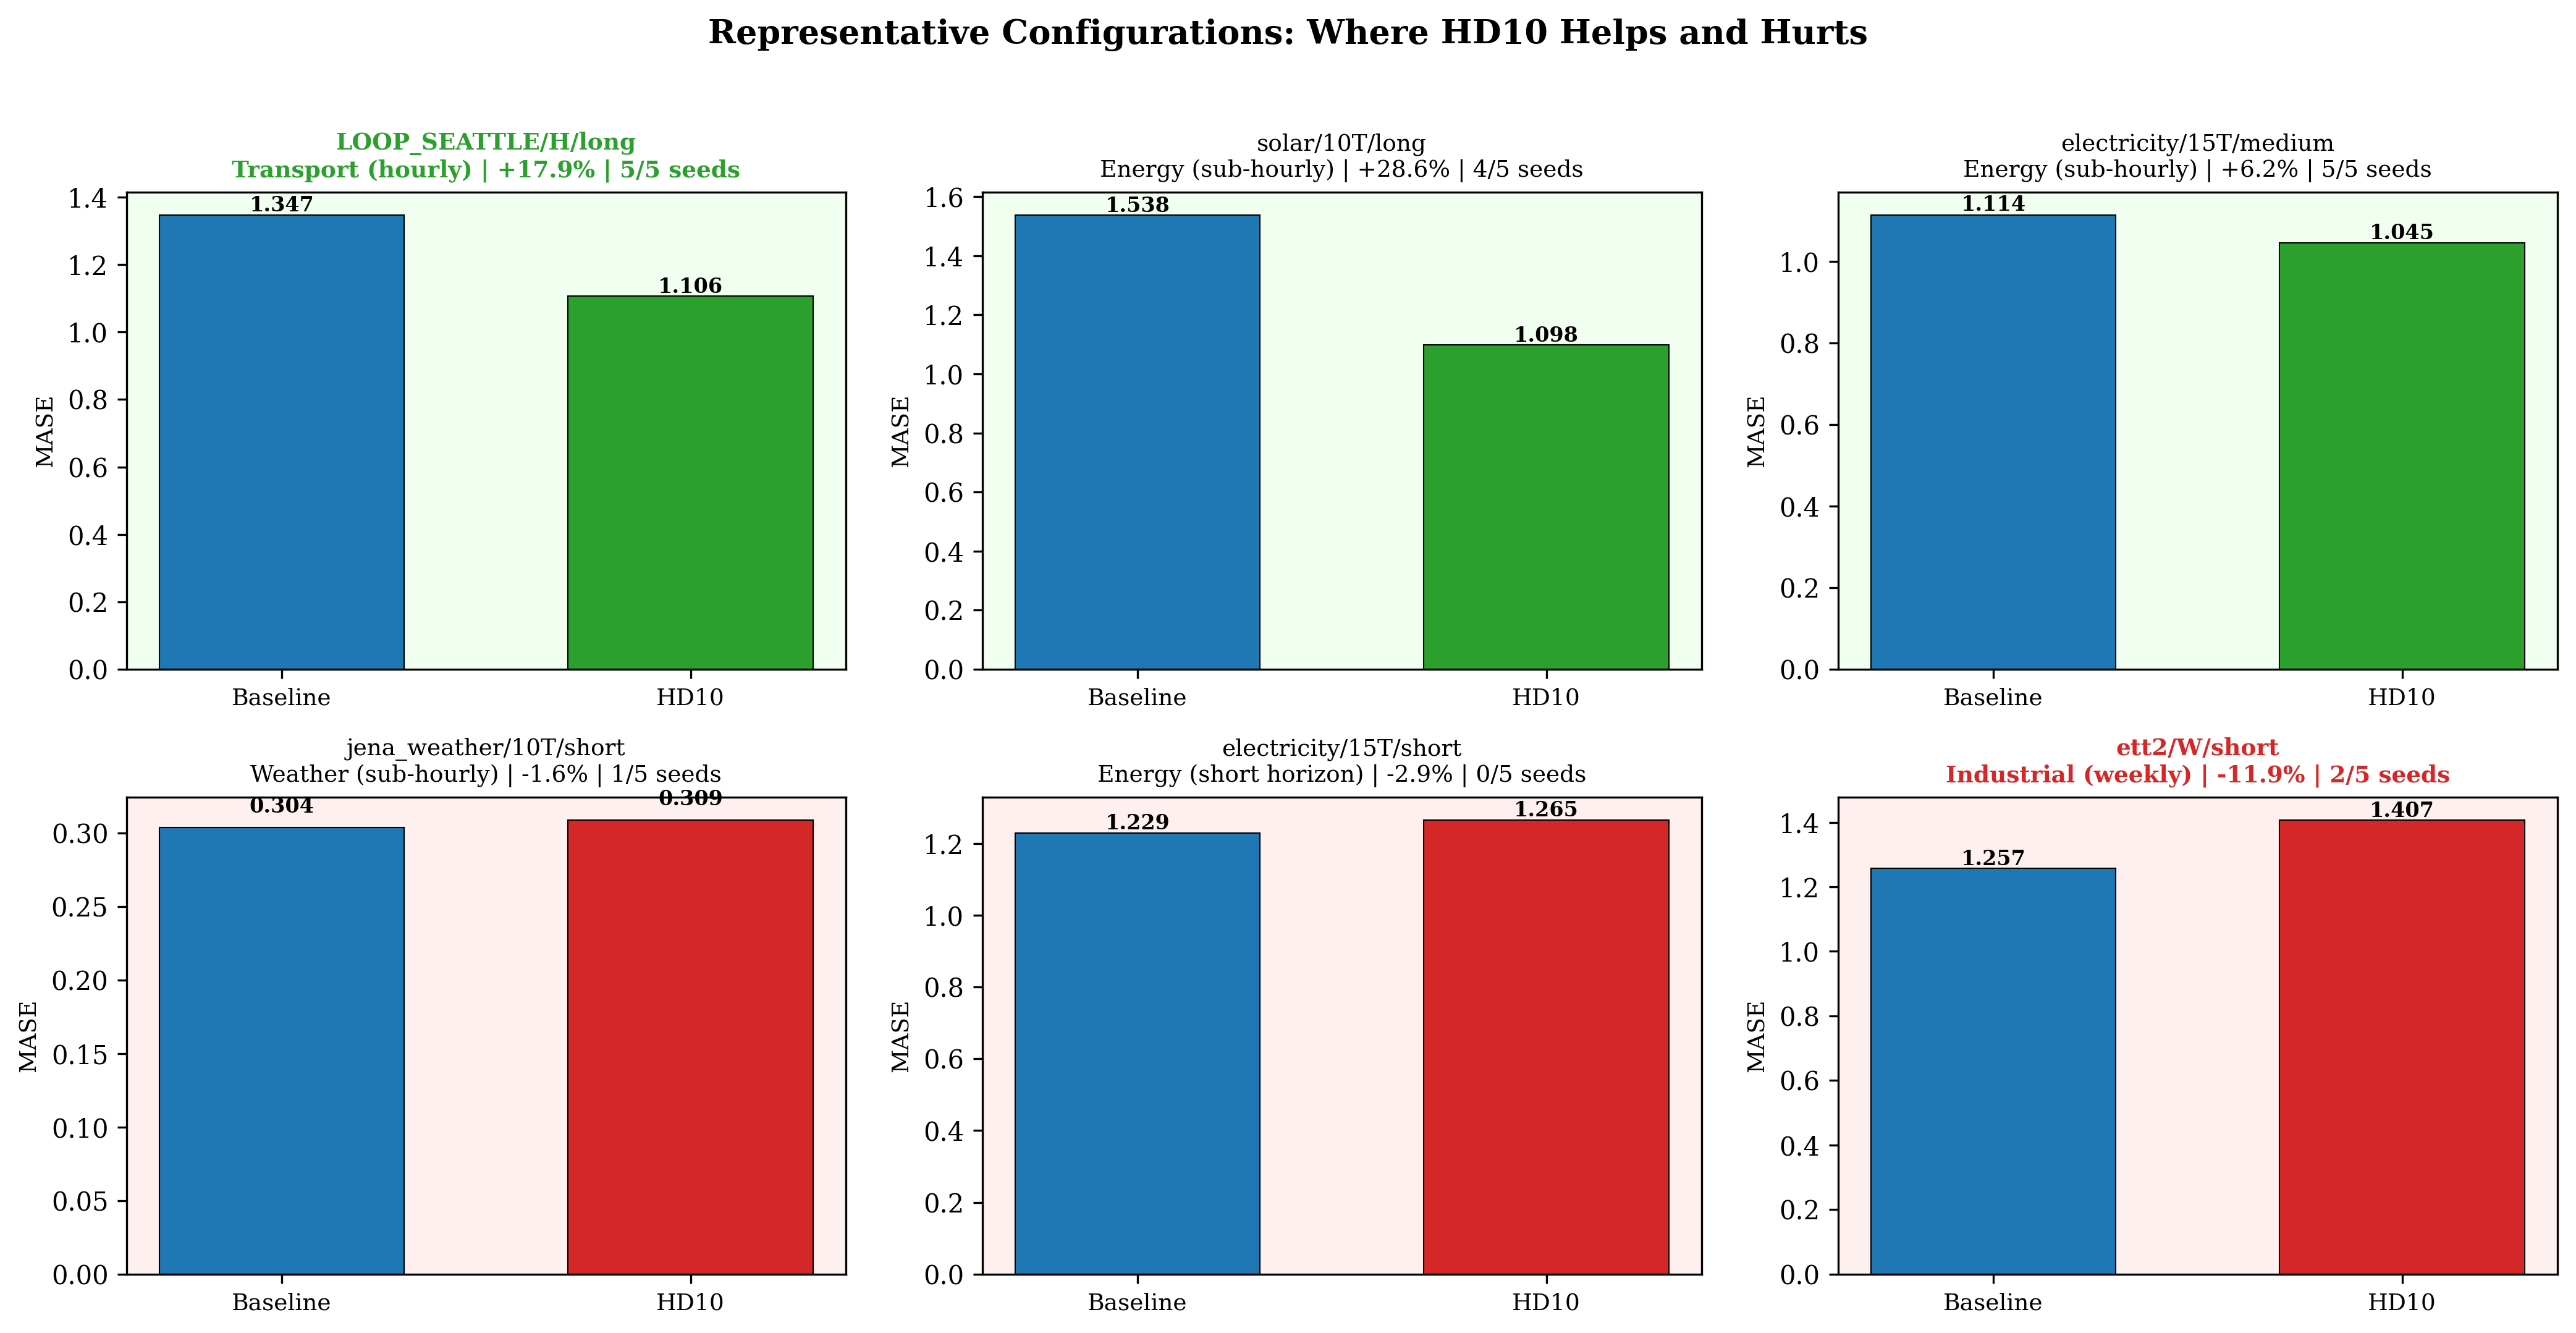
\includegraphics[width=\linewidth]{figures/fig_qualitative_configs.pdf}
\caption{Six representative configurations spanning the range of HD10 performance. Top row: strong wins (transport, energy). Bottom row: neutral (weather) and losses (short horizon, weekly).}
\end{figure}

\subsection{Full Configuration Heatmap}

\begin{figure}[h]
\centering
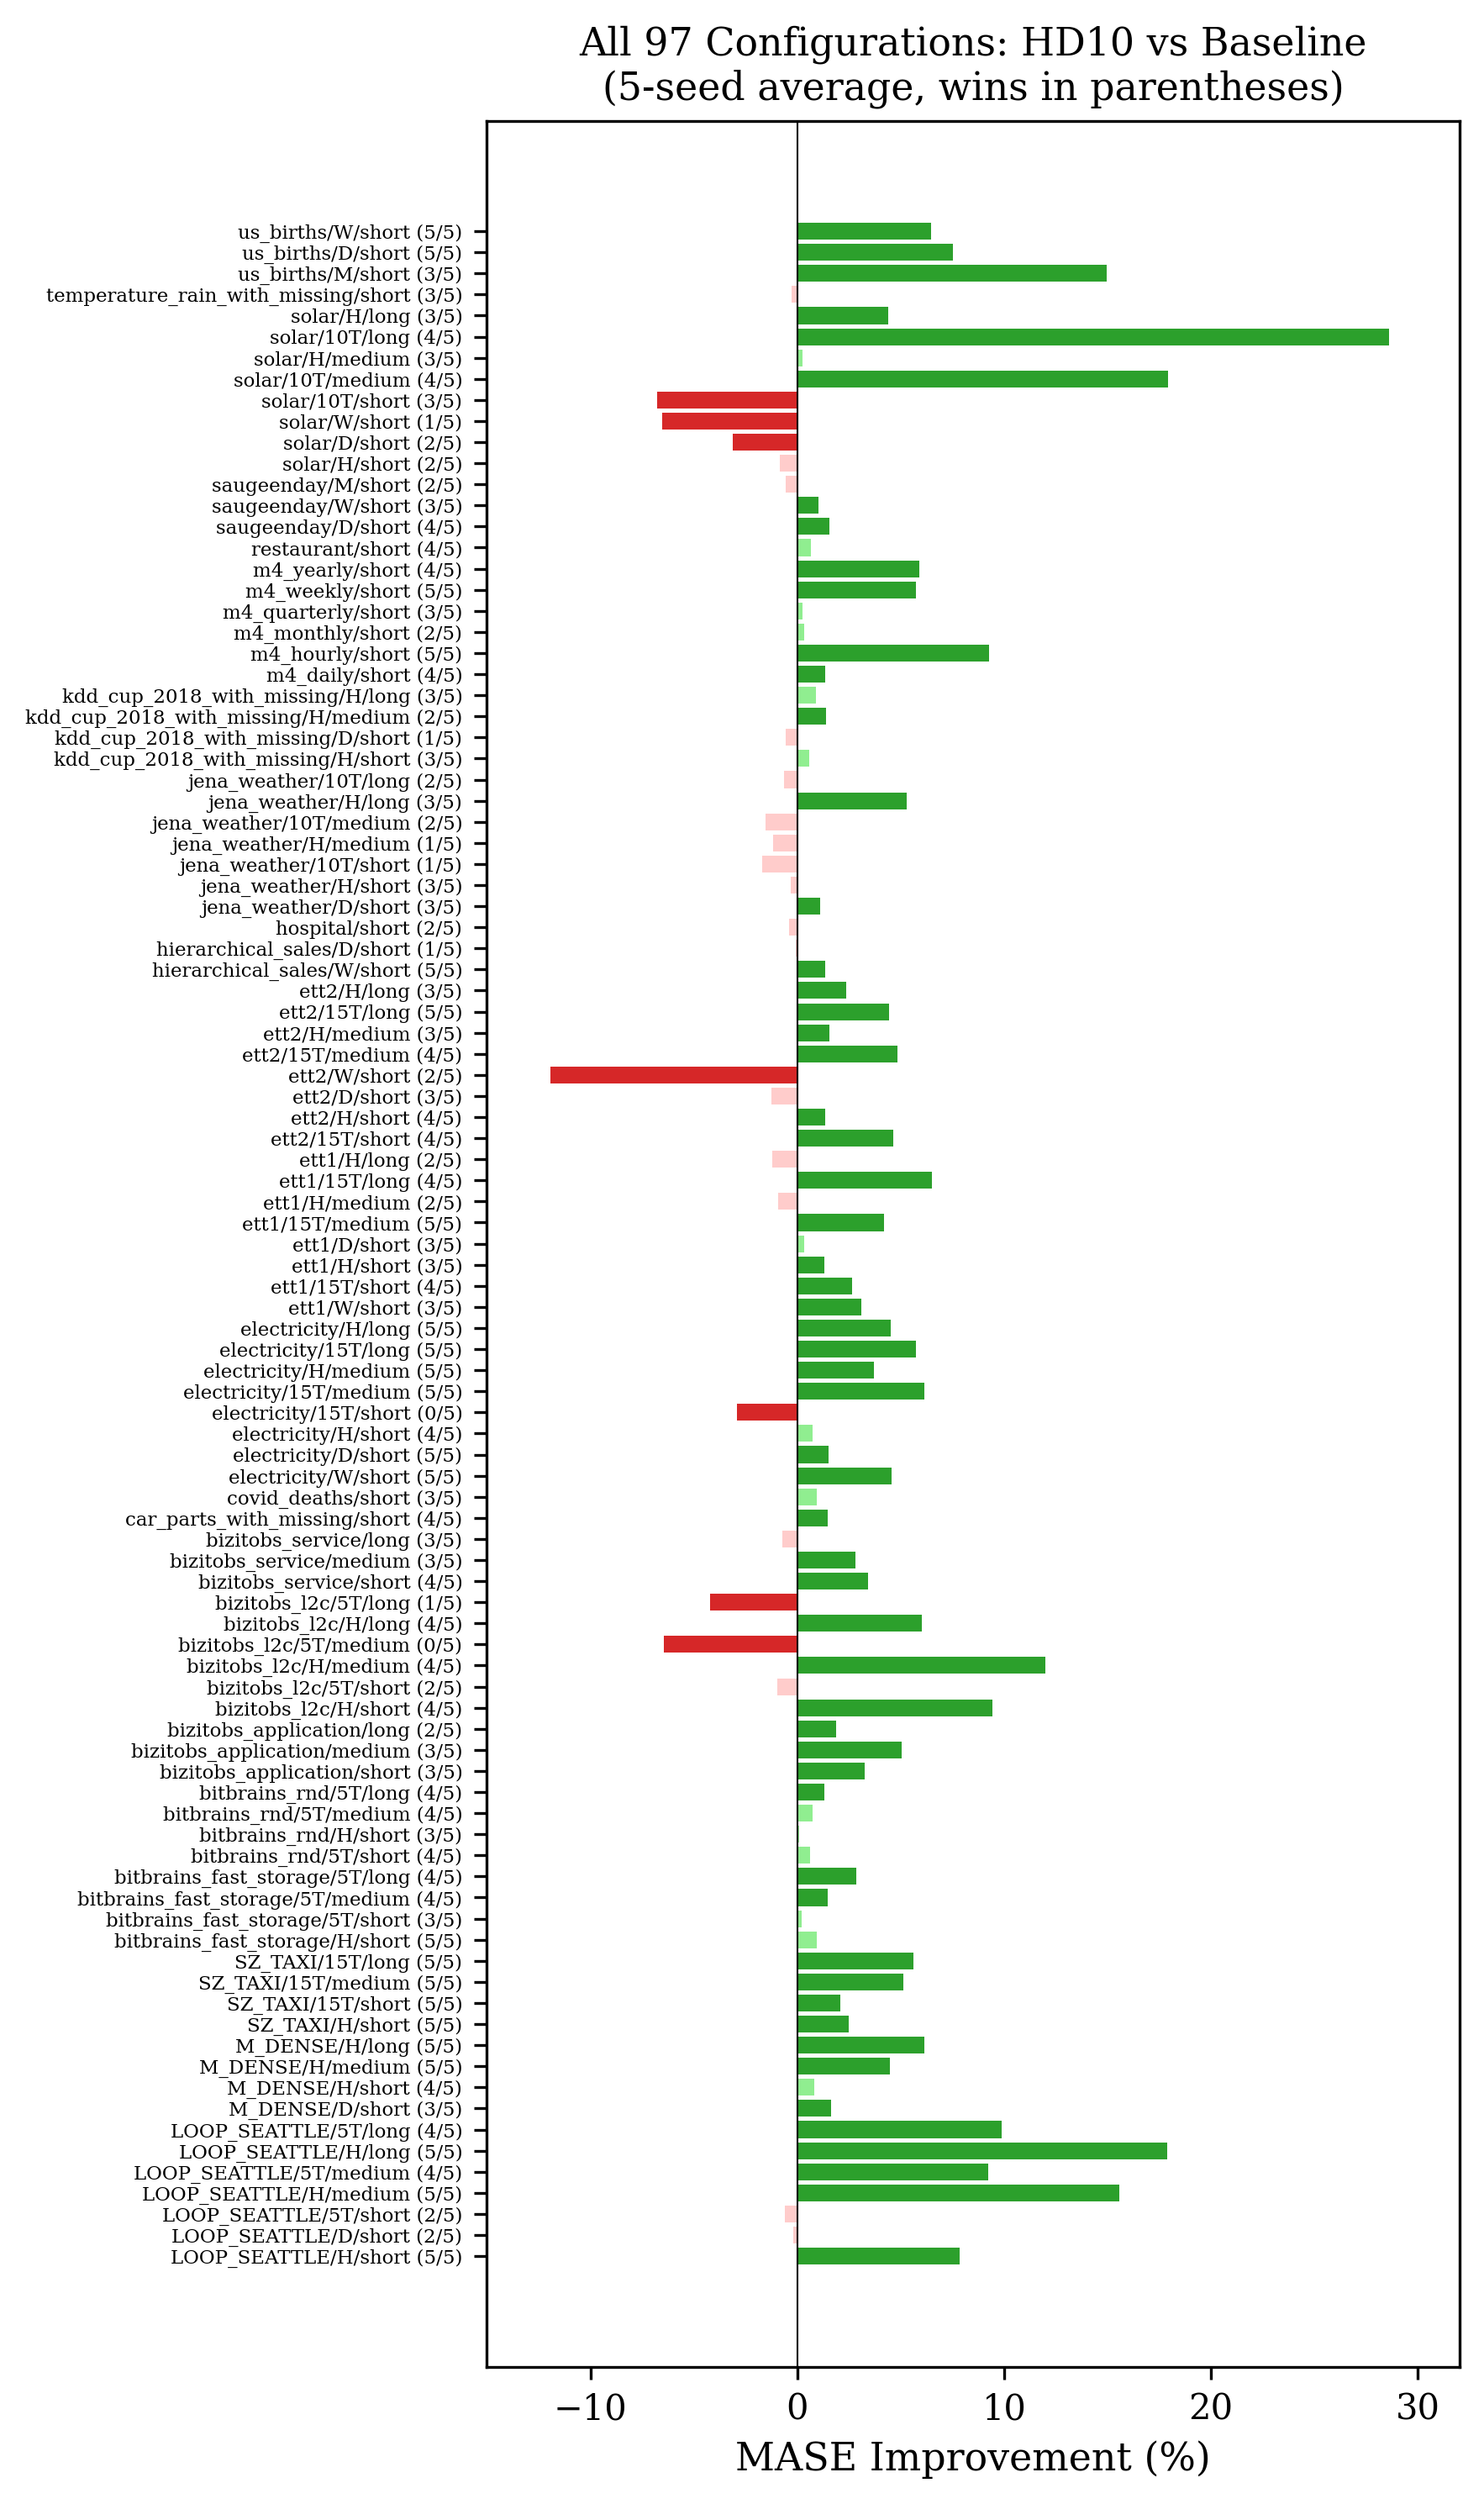
\includegraphics[width=0.55\linewidth]{figures/fig_full_heatmap.pdf}
\caption{All 97 configurations sorted by dataset, showing 5-seed averaged improvement and seed win count. Dark green: strong improvement. Red: regression.}
\end{figure}

\subsection{Pending Experiments}

The following experiments have been submitted and are awaiting results:

\begin{itemize}
    \item \textbf{HD0}: Chebyshev $d=4$, $s=16$, 0\% dropout (5 seeds), completing the dropout ablation
    \item \textbf{Dup/Zero at $\eta = 2 \times 10^{-3}$}: Capacity controls at matched optimal LR (5 seeds each)
    \item \textbf{Dup/Zero at 100K}: Capacity controls at full training budget (3 seeds each)
    \item \textbf{LR control 100K}: Baseline and HD10 with cosine-floor ($\eta_{\min} = 0.1\eta_{\max}$) and WSD schedule
    \item \textbf{Official Moirai-2 eval}: HuggingFace checkpoint evaluated on GIFT-Eval for calibration
\end{itemize}

\end{document}
